% A LaTeX template for MSc Thesis submissions to 
% Politecnico di Milano (PoliMi) - School of Industrial and Information Engineering
%
% S. Bonetti, A. Gruttadauria, G. Mescolini, A. Zingaro
% e-mail: template-tesi-ingind@polimi.it
%
% Last Revision: October 2021
%
% Copyright 2021 Politecnico di Milano, Italy. NC-BY

\documentclass{Configuration_Files/PoliMi3i_thesis}

%------------------------------------------------------------------------------
%	REQUIRED PACKAGES AND  CONFIGURATIONS
%------------------------------------------------------------------------------

% CONFIGURATIONS
\usepackage{multirow}
\usepackage{pdflscape}
\usepackage{lscape}
\usepackage{parskip} % For paragraph layout
\usepackage{setspace} % For using single or double spacing
\usepackage{emptypage} % To insert empty pages
\usepackage{multicol} % To write in multiple columns (executive summary)
\setlength\columnsep{15pt} % Column separation in executive summary
\setlength\parindent{0pt} % Indentation
\raggedbottom  

% PACKAGES FOR TITLES
\usepackage{titlesec}
% \titlespacing{\section}{left spacing}{before spacing}{after spacing}
\titlespacing{\section}{0pt}{3.3ex}{2ex}
\titlespacing{\subsection}{0pt}{3.3ex}{1.65ex}
\titlespacing{\subsubsection}{0pt}{3.3ex}{1ex}
\usepackage{color}

% PACKAGES FOR LANGUAGE AND FONT
\usepackage[english]{babel} % The document is in English  
\usepackage[utf8]{inputenc} % UTF8 encoding
\usepackage[T1]{fontenc} % Font encoding
\usepackage[11pt]{moresize} % Big fonts

% PACKAGES FOR IMAGES
 \usepackage{epigraph}
%\usepackage{subcaption}
\usepackage{graphicx}
\usepackage{transparent} % Enables transparent images
\usepackage{eso-pic} % For the background picture on the title page
\usepackage{subfig} % Numbered and caption subfigures using \subfloat.
\usepackage{tikz} % A package for high-quality hand-made figures.
\usetikzlibrary{}
\graphicspath{{./Images/}} % Directory of the images
\usepackage{caption} % Coloured captions
\usepackage{xcolor} % Coloured captions
\usepackage{amsthm,thmtools,xcolor} % Coloured "Theorem"
\usepackage{float}

% STANDARD MATH PACKAGES
\usepackage{amsmath}
\usepackage{amsthm}
\usepackage{amssymb}
\usepackage{amsfonts}
\usepackage{bm}
\usepackage[overload]{empheq} % For braced-style systems of equations.
\usepackage{fix-cm} % To override original LaTeX restrictions on sizes

% PACKAGES FOR TABLES
\usepackage{tabularx}
\usepackage{longtable} % Tables that can span several pages
\usepackage{colortbl}

% PACKAGES FOR ALGORITHMS (PSEUDO-CODE)
\usepackage{algorithm}
\usepackage{algorithmic}

% PACKAGES FOR REFERENCES & BIBLIOGRAPHY
\usepackage[colorlinks=true,linkcolor=black,anchorcolor=black,citecolor=black,filecolor=black,menucolor=black,runcolor=black,urlcolor=black]{hyperref} % Adds clickable links at references
\usepackage{cleveref}
\usepackage[square, numbers, sort&compress]{natbib} % Square brackets, citing references with numbers, citations sorted by appearance in the text and compressed
\bibliographystyle{abbrvnat} % You may use a different style adapted to your field

% OTHER PACKAGES
\usepackage{pdfpages} % To include a pdf file
\usepackage{afterpage}
\usepackage{lipsum} % DUMMY PACKAGE
\usepackage{fancyhdr} % For the headers
\fancyhf{}

% Input of configuration file. Do not change config.tex file unless you really know what you are doing. 
% Define blue color typical of polimi
\definecolor{bluepoli}{cmyk}{0.4,0.1,0,0.4}

% Custom theorem environments
\declaretheoremstyle[
  headfont=\color{bluepoli}\normalfont\bfseries,
  bodyfont=\color{black}\normalfont\itshape,
]{colored}

% Set-up caption colors
\captionsetup[figure]{labelfont={color=bluepoli}} % Set colour of the captions
\captionsetup[table]{labelfont={color=bluepoli}} % Set colour of the captions
\captionsetup[algorithm]{labelfont={color=bluepoli}} % Set colour of the captions

\theoremstyle{colored}
\newtheorem{theorem}{Theorem}[chapter]
\newtheorem{proposition}{Proposition}[chapter]

% Enhances the features of the standard "table" and "tabular" environments.
\newcommand\T{\rule{0pt}{2.6ex}}
\newcommand\B{\rule[-1.2ex]{0pt}{0pt}}

% Pseudo-code algorithm descriptions.
\newcounter{algsubstate}
\renewcommand{\thealgsubstate}{\alph{algsubstate}}
\newenvironment{algsubstates}
  {\setcounter{algsubstate}{0}%
   \renewcommand{\STATE}{%
     \stepcounter{algsubstate}%
     \Statex {\small\thealgsubstate:}\space}}
  {}

% New font size
\newcommand\numfontsize{\@setfontsize\Huge{200}{60}}

% Title format: chapter
\titleformat{\chapter}[hang]{
\fontsize{50}{20}\selectfont\bfseries\filright}{\textcolor{bluepoli} \thechapter\hsp\hspace{2mm}\textcolor{bluepoli}{|   }\hsp}{0pt}{\huge\bfseries \textcolor{bluepoli}
}

% Title format: section
\titleformat{\section}
{\color{bluepoli}\normalfont\Large\bfseries}
{\color{bluepoli}\thesection.}{1em}{}

% Title format: subsection
\titleformat{\subsection}
{\color{bluepoli}\normalfont\large\bfseries}
{\color{bluepoli}\thesubsection.}{1em}{}

% Title format: subsubsection
\titleformat{\subsubsection}
{\color{bluepoli}\normalfont\large\bfseries}
{\color{bluepoli}\thesubsubsection.}{1em}{}

% Shortening for setting no horizontal-spacing
\newcommand{\hsp}{\hspace{0pt}}

\makeatletter
% Renewcommand: cleardoublepage including the background pic
\renewcommand*\cleardoublepage{%
  \clearpage\if@twoside\ifodd\c@page\else
  \null
  \AddToShipoutPicture*{\BackgroundPic}
  \thispagestyle{empty}%
  \newpage
  \if@twocolumn\hbox{}\newpage\fi\fi\fi}
\makeatother

%For correctly numbering algorithms
\numberwithin{algorithm}{chapter}

%----------------------------------------------------------------------------
%	NEW COMMANDS DEFINED
%----------------------------------------------------------------------------

% EXAMPLES OF NEW COMMANDS
\newcommand{\bea}{\begin{eqnarray}} % Shortcut for equation arrays
\newcommand{\eea}{\end{eqnarray}}
\newcommand{\e}[1]{\times 10^{#1}}  % Powers of 10 notation

%----------------------------------------------------------------------------
%	ADD YOUR PACKAGES (be careful of package interaction)
%----------------------------------------------------------------------------

%----------------------------------------------------------------------------
%	ADD YOUR DEFINITIONS AND COMMANDS (be careful of existing commands)
%----------------------------------------------------------------------------

%----------------------------------------------------------------------------
%	BEGIN OF YOUR DOCUMENT
%----------------------------------------------------------------------------

\begin{document}

\fancypagestyle{plain}{%
\fancyhf{} % Clear all header and footer fields
\fancyhead[RO,RE]{\thepage} %RO=right odd, RE=right even
\renewcommand{\headrulewidth}{0pt}
\renewcommand{\footrulewidth}{0pt}}

%----------------------------------------------------------------------------
%	TITLE PAGE
%----------------------------------------------------------------------------

\pagestyle{empty} % No page numbers
\frontmatter % Use roman page numbering style (i, ii, iii, iv...) for the preamble pages

\puttitle{
	title=  Public transport service \\for the new Business Park in Stradella, % Title of the thesis
	name=\\ 
	      \vspace{0.2 cm}\\
	      Chiara Beretta \hspace{1,15 cm}
          Fabio Cassanmagnago \hspace{2,2 cm} 
          Luca Cattaneo \\ 
          \vspace{0.001 cm}\\          
          Dario Dodi \hspace{1,95 cm}  
          Francesco Manzoni \hspace{2,79 cm}  
          Fabio Vitiello  ,, % Author Name and Surname
	course= Public Transport Management \\(M.Sc.) Mobility Engineering, % Study Programme (in Italian)
	advisor= Prof. Name Surname, % Supervisor name
	coadvisor={Name Surname, Name Surname}, % Co-Supervisor name, remove this line if there is none
	academicyear={2021-2022},  % Academic Year
} % These info will be put into your Title page 

%----------------------------------------------------------------------------
%	PREAMBLE PAGES: ABSTRACT (inglese e italiano), EXECUTIVE SUMMARY
%----------------------------------------------------------------------------
\startpreamble
\setcounter{page}{1} % Set page counter to 1

%----------------------------------------------------------------------------
%	LIST OF CONTENTS/FIGURES/TABLES/SYMBOLS
%----------------------------------------------------------------------------

% TABLE OF CONTENTS
\thispagestyle{empty}
\tableofcontents % Table of contents 
\thispagestyle{empty}
\cleardoublepage

%-------------------------------------------------------------------------
%	THESIS MAIN TEXT
%-------------------------------------------------------------------------
% In the main text of your thesis you can write the chapters in two different ways:
%
%(1) As presented in this template you can write:
%    \chapter{Title of the chapter}
%    *body of the chapter*
%
%(2) You can write your chapter in a separated .tex file and then include it in the main file with the following command:
%    \chapter{Title of the chapter}
%    \input{chapter_file.tex}
%
% Especially for long thesis, we recommend you the second option.

\addtocontents{toc}{\vspace{2em}} % Add a gap in the Contents, for aesthetics
\mainmatter % Begin numeric (1,2,3...) page numbering

% --------------------------------------------------------------------------
% NUMBERED CHAPTERS % Regular chapters following
% --------------------------------------------------------------------------
\chapter{Introduction}
The objective of this project course is to re-design a bus public transport service for one of the new biggest working poles in the Pavia area: the business park in Stradella.

This rural territory is living an intense sub-urban commercial re-development process from the last 5 years thanks to both its high availability of commercial buildable lands and its proximity to mobility infrastructure. In fact, the area not only offers the direct access to the A21 “Wine highway”, many capillary freeways and the railway infrastructure network, but also has a strategic proximity to many important cities such as Milan (60 km) ,  Pavia (20 km), Cremona (50 km),  Alessandria (60 km), Parma (100 km), Turin (150km) and the Genova harbor (115 km).

This higher and higher industrial activities development needs more and more manpower availability, and thus creating a huge accessibility demand for the employees. Estimated around for 2000 people per day, this labor mobility needs has mainly two sources of demand fragmentations: a temporal and spatial one. The first feature is given by the different working time of the operating companies, which could be organized according to a full-day working time – 24 hours per day by 3 working shifts at 6, 14 and 22. – or by a more traditional daily-time working schedule from 8.30 to 17.30  Instead, the second fragmentation feature is given by the manpower residential spatial location, which is not limited to the Stradella area – which count only 11’600 inhabitants- but also on the surrounding cities of Broni, Voghera, Pavia, Casteggio and Castel San Giovanni.

The combination of these two fragmentation demand sources with an actual absence of a tailored public transport service able to answer to the new business park mobility needs, could easily lead to car-oriented employees modal choice: unsustainable on the long period both on the environmental and traffic side. Aware of this possible oncoming problem, the local Public Administration has expressed its interest in the renovation of the public transport service on that area in according with the raising demand for that service from the employees too – estimated for more than the $10\%$ of the total manpower.

After an in-depth analysis of the business park area, its current public transport service’s offer and the “new” employee’s mobility demand needs, we will focus on the possible ways to match them proposing new public transport solutions, acting both on the actual line side and studying new ones. All these new proposals will be analyzed from the top planning level –lines features- until the ordinary daily operation detail – sizing and scheduling of the service- in a consistent way, by the usage of a technical and an economic analysis to ensure the service overall sustainability. The last step will take into consideration the market launch strategy to find effective ways to promote and diffuse the new service awareness and its benefit among all the business park’s employees. 

\chapter{Demand Offer Analysis}
The first step of the project work is dedicated to the analysis of the current public transport offer and of the demand of the Business Park. Firstly, in the section \ref{sec:offer} it is represented the current offer with the use of QGIS, then there is the identification of the useful rides and loads in the paragraph 1.2. The paragraph 1.3 illustrates the representation of the demand and the preferences of mean of transport of the workers from and to the Business Park. The output of this first part is reported in the paragraph 1.4 with the evaluation of the capacity of the current service to satisfy the demand and the identification of proposal of service enhancements, which will be defined in detail in the next phase.

\section{Represent the current offer}
\label{sec:offer}
With the use of QGIS the actual state of the offer is represented. The \ref{fig:offer} shows all the lines.

\begin{figure}[ht]
    \centering
    \includegraphics[width=0.7\textwidth]{Images/demand_offer_analysis/Lines.png}
    \caption{The actual offer}
    \label{fig:offer}
\end{figure}

Now in Figure \ref{fig:rail} railway infrastructure from ORM is presented.

\begin{figure}[h]
    \centering
    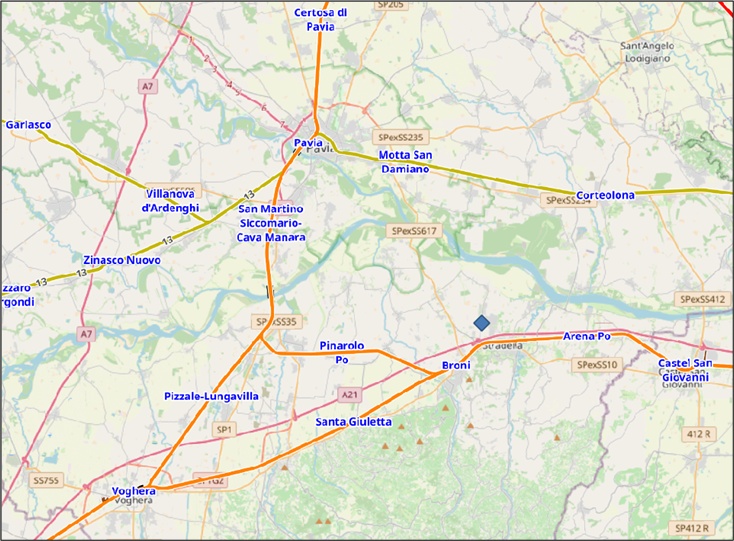
\includegraphics[width=0.7\textwidth]{Images/demand_offer_analysis/railway.png}
    \caption{The railway infrastructure from ORM}
    \label{fig:rail}
\end{figure}

So, there are railway infrastructure between:

\begin{itemize}
    \item Pavia – Voghera
    \item Voghera- Broni- Stradella - Castel San Giovanni
    \item Pavia – Broni -Stradella – Castel San Giovanni
\end{itemize}
In the analysis of the different timeslots will be also considered the connection with railway service to assess the feasibility of an intermodal approach.

Then with the use of a Python script (algorithm \ref{alg:var}) has been represented the offer in different time slots. It has been considered the departure time from the first stop to be included in the timeslot.

As can be seen in the Figure \ref{fig:offer56} only line P132, P184, P085, P098 have a departure between 05:00 and 06:00.

In Figure \ref{fig:offer730830} Line P095 has two rides that  start between 07:30 and 08:30 \footnote{Note that the result contains all the rides that have a departure between 07:30 and 08:30 but the end time has not been considered. So, a bus can start at 08:25 and it will be considered in the time slot. The analysis would be deepened in the following of the report}.Instead, lines P132, P410, P182, P133, P98, P430 and P095 have only one ride.

In Figure \ref{fig:offer13} the offer increases, because it is the time of exit from school, and a capillary network has been founded with lines P095,P098,P132,P133,P179,P182,P184,P410 and P430 having also a ride that starts in this timeslots.

\begin{figure}
\centering
\subfloat[Lines with departure between 05:00 and 06:00]{\label{fig:offer56}{\includegraphics[width=0.6\textwidth]{Images/demand_offer_analysis/Routes_5_6.png}}}\hfill

\subfloat[Lines with departure between 07:30 and 08:30]{\label{fig:offer730830}{\includegraphics[width=0.6\textwidth]{Images/demand_offer_analysis/730-830.png}}}

\subfloat[Lines with rides that depart between 13 and 14]{\label{fig:offer13}{\includegraphics[width=0.6\textwidth]{Images/demand_offer_analysis/13-14.png}}}
\end{figure}

\subsection{Recap on the representation of the offer}
From the analysis it seems that maximum a ride per hour is scheduled. There is no report about the timeslot 21-23 because there are not any rides. For the timeslot 17:30-18:30 the situation is similar to the 07:30-8:30 with the line P95 with higher number of departure.
In addition, after a look to the railway services timetables the intermodal approach is not feasible. This will now argued with an example: considering the shift 06:00-14:00, the train should arrive to Stradella FS at 05:30 to make possible a connection by bus with the Business Park. But looking to the timetables there are not any train rides compatible with that schedule. This makes unfeasible creating an intermodal connection also for the exit time at 14:00, because the workers would arrive at work by bus in the morning, but they would come back with train. This will imply a more complex ticketing system for the users.
 
In other words, an intermodal approach is feasible if can be adopted for entry time and for exit time and for all the shifts. In this case this cannot be applied so in the next sections will be considered only transport by buses.

\section{«Useful» rides and loads}

To evaluate the capacity of the current offer to satisfy the demand it is necessary to identify the useful rides for reaching the business park in each time slot of interest.
In this step of the analysis is not considered yet the demand of mobility in the different areas and the preferences of the customers, that will be included in the next paragraphs.

The useful rides have two characteristics:

\begin{itemize}
    \item Have a compatible route with a terminus or transit near the business park, in order to require only an extension or a deviation of few kilometers
    \item Have a compatible arrival time with the entry time of the workers or require only a slight modification of the timetable
\end{itemize}

The Table \ref{tab:loads} represents the useful rides for each time slot. In the last column of the table is reported also the rides’ loads. The total capacity of the buses is 56 seats due to covid restrictions and some rides’ loads are not available.

For what concern the entry of the worker at 6 in the morning there are not any useful rides, because with an arrival time near the business park too late or too soon, or because they have not a compatible route.

For the entry and the exit of the workers at 22 there are not any rides in those time slots, so not even useful rides.
\newpage
% Please add the following required packages to your document preamble:
% \usepackage[table,xcdraw]{xcolor}
% If you use beamer only pass "xcolor=table" option, i.e. \documentclass[xcolor=table]{beamer}
\newpage
\thispagestyle{empty}
\begin{landscape}
\begin{table}[ht]
\centering
\begin{tabular}{|llllll|}
\hline
\rowcolor{bluepoli!40}
\multicolumn{1}{|c|}{\textbf{Line}} & \multicolumn{1}{c|}{{\color[HTML]{333333} \textbf{Ride code}}} & \multicolumn{1}{c|}{{\color[HTML]{333333} \textbf{Departure   time}}} & \multicolumn{1}{c|}{{\color[HTML]{333333} \textbf{Arrival time}}} & \multicolumn{1}{c|}{{\color[HTML]{333333} \textbf{Route   description}}}  & \multicolumn{1}{c|}{{\color[HTML]{333333} \textbf{Loads}}} \\ \hline
\multicolumn{6}{|c|}{Entry 8.30}                                                                                                                                                                                                                                                                                                                                                          \\ \hline
\multicolumn{1}{|l|}{P095+A2:I3}    & \multicolumn{1}{l|}{195099}                                    & \multicolumn{1}{l|}{07:35}                                            & \multicolumn{1}{l|}{08:06}                                        & \multicolumn{1}{l|}{C.S.GIOV. Gramsci   STRADELLA   BRONI Emilia, 366}    & 8\%                                                        \\ \hline
\multicolumn{1}{|l|}{PV95}          & \multicolumn{1}{l|}{195062}                                    & \multicolumn{1}{l|}{07:40}                                            & \multicolumn{1}{l|}{08:11}                                        & \multicolumn{1}{l|}{C.S.GIOV. Gramsci   STRADELLA   BRONI   Emilia, 366}  & 5\%                                                        \\ \hline
\multicolumn{1}{|l|}{PV95}          & \multicolumn{1}{l|}{195011}                                    & \multicolumn{1}{l|}{07:45}                                            & \multicolumn{1}{l|}{08:35}                                        & \multicolumn{1}{l|}{PV Aut.   P.te Becca   BRONI   STRADELLA Allea}       & 25\%                                                       \\ \hline
\multicolumn{1}{|l|}{PV10010}       & \multicolumn{1}{l|}{410003}                                    & \multicolumn{1}{l|}{07:30}                                            & \multicolumn{1}{l|}{08:02}                                        & \multicolumn{1}{l|}{S.MARIA V.Veneto   STRADELLA   BRONI   Emilia/Italia} & -                                                          \\ \hline
\multicolumn{6}{|c|}{Entry 14}                                                                                                                                                                                                                                                                                                                                                            \\ \hline
\multicolumn{1}{|l|}{PV95}          & \multicolumn{1}{l|}{195025}                                    & \multicolumn{1}{l|}{13:00}                                            & \multicolumn{1}{l|}{13:50}                                        & \multicolumn{1}{l|}{PV Aut.   BRONI   STRADELLA Allea}                    & 45\%                                                       \\ \hline
\multicolumn{1}{|l|}{PV95}          & \multicolumn{1}{l|}{195113}                                    & \multicolumn{1}{l|}{13:09}                                            & \multicolumn{1}{l|}{14:16}                                        & \multicolumn{1}{l|}{C.S.GIOV   STRADELLA   BRONI   PV Aut}                & 75\%                                                       \\ \hline
\multicolumn{1}{|l|}{PV132}         & \multicolumn{1}{l|}{132028}                                    & \multicolumn{1}{l|}{13:10}                                            & \multicolumn{1}{l|}{14:04}                                        & \multicolumn{1}{l|}{VOGHERA   CASTEG FS   BRONI Italia     STRADELLA FS}  & -                                                          \\ \hline
\multicolumn{6}{|c|}{Exit 6}                                                                                                                                                                                                                                                                                                                                                              \\ \hline
\multicolumn{1}{|l|}{PV132}         & \multicolumn{1}{l|}{132003}                                    & \multicolumn{1}{l|}{06:45}                                            & \multicolumn{1}{l|}{07:40}                                        & \multicolumn{1}{l|}{STRAD FS   BRONI Italia   CASTEG FS     VOGHERA}      & 53\%                                                       \\ \hline
\multicolumn{1}{|l|}{PV95}          & \multicolumn{1}{l|}{195153}                                    & \multicolumn{1}{l|}{06:30}                                            & \multicolumn{1}{l|}{07:43}                                        & \multicolumn{1}{l|}{STRAD Battisti   BRONI   P.Becca   MI FAMM2}          & 4\%                                                        \\ \hline
\multicolumn{6}{|c|}{Exit 14}                                                                                                                                                                                                                                                                                                                                                             \\ \hline
\multicolumn{1}{|l|}{PV95}          & \multicolumn{1}{l|}{195031}                                    & \multicolumn{1}{l|}{13:55}                                            & \multicolumn{1}{l|}{14:24}                                        & \multicolumn{1}{l|}{BRONI  C.S.GIOV. Gramsci}                             & 18\%                                                       \\ \hline
\multicolumn{1}{|l|}{PV10040}       & \multicolumn{1}{l|}{440010}                                    & \multicolumn{1}{l|}{13:57}                                            & \multicolumn{1}{l|}{14:45}                                        & \multicolumn{1}{l|}{BRONI   STR V.Ven   CASTAN     S.MARIA V.Ven}         & -                                                          \\ \hline
\multicolumn{1}{|l|}{PV95}          & \multicolumn{1}{l|}{195152}                                    & \multicolumn{1}{l|}{14:00}                                            & \multicolumn{1}{l|}{15:04}                                        & \multicolumn{1}{l|}{PV Aut.   BRONI   STRAD     C.S.GIOV Gramsci}         & 49\%                                                       \\ \hline
\multicolumn{1}{|l|}{PV10010}       & \multicolumn{1}{l|}{410027}                                    & \multicolumn{1}{l|}{14:09}                                            & \multicolumn{1}{l|}{14:40}                                        & \multicolumn{1}{l|}{BRONI   STRADELLA   S.MARIA V.Veneto}                 & -                                                          \\ \hline
\multicolumn{1}{|l|}{PV80}          & \multicolumn{1}{l|}{80032}                                     & \multicolumn{1}{l|}{14:10}                                            & \multicolumn{1}{l|}{15:02}                                        & \multicolumn{1}{l|}{STRA Batt BRO Italia . CASTEGGIO FS}                  & -                                                          \\ \hline
\multicolumn{1}{|l|}{PV132}         & \multicolumn{1}{l|}{132031}                                    & \multicolumn{1}{l|}{14:15}                                            & \multicolumn{1}{l|}{15:03}                                        & \multicolumn{1}{l|}{STRADELLA FS   BRONI Italia   VOGHERA   Aut.}         & 52\%                                                       \\ \hline
\multicolumn{1}{|l|}{PV95}          & \multicolumn{1}{l|}{195119}                                    & \multicolumn{1}{l|}{14:40}                                            & \multicolumn{1}{l|}{15:27}                                        & \multicolumn{1}{l|}{STRADELLA Trieste   BRONI   P.te Becca   PAV Aut.}    & 18\%                                                       \\ \hline
\multicolumn{1}{|l|}{PV10010}       & \multicolumn{1}{l|}{410022}                                    & \multicolumn{1}{l|}{14:45}                                            & \multicolumn{1}{l|}{15:20}                                        & \multicolumn{1}{l|}{BRONI Ita   STR V.Ven   S.MARIA V.Veneto}             & -                                                          \\ \hline
\multicolumn{6}{|c|}{Exit 17.30}                                                                                                                                                                                                                                                                                                                                                          \\ \hline
\multicolumn{1}{|l|}{PV184}         & \multicolumn{1}{l|}{184033}                                    & \multicolumn{1}{l|}{17:50}                                            & \multicolumn{1}{l|}{19:05}                                        & \multicolumn{1}{l|}{STRADELLA Battisti   CALV B.PRI   CASTEGGIO}          & -                                                          \\ \hline
\multicolumn{1}{|l|}{PV85}          & \multicolumn{1}{l|}{85020}                                     & \multicolumn{1}{l|}{17:55}                                            & \multicolumn{1}{l|}{19:18}                                        & \multicolumn{1}{l|}{STRAD V.Ven   S.MARIA V   ROMAGNESE Pesa}             & -                                                          \\ \hline
\end{tabular}
\caption{Useful rides}
\label{tab:loads}
\end{table}
\end{landscape}
\newpage
\newpage
\section{Demand}

The analysis is based on an Excel file that contains two worksheets about the weighted number of the shifts\footnote{he workers change the shifts by days, so the demand is weighted to have a real estimation of the demand. The daytime is not weighted because is fix.}  and the preferences of means of transport.
There are four work shifts:

\begin{itemize}
    \item 06:00-14:00
    \item 14:00-22:00
    \item 22:00-06:00
    \item 08:30-17:30
\end{itemize}
So given the provided data and the shapefile \cite{Istat2022CONFINI2022} the demand has been plotted.

\paragraph{Demand shift 06:00 - 14:00}

Figure \ref{fig:demand614} represents the desired lines based on the demand.

The municipalities in the zone with the lowest demand are not considered because their demand is too low and with high preference for private car.

Stradella and Broni represent the municipalities with highest demand. They are also the ones with lowest willingness to use the public transport. This because they are the nearest to the Business Park. Nevertheless, the number of people that will use the public transport justifies taking them in consideration. 

Following a similar reasoning also Voghera should be considered.

Surprisingly Pavia has the same level of demand of Casteggio and Castel San Giovanni. Those municipality whose demand is the second lowest should be considered only if this do not require important changes of the services.

\paragraph{Demand shift 14:00 - 22:00}
Pavia, Casteggio and Castel San Giovanni remain with the same level of demand and for this reason will be considered only if the changes will not impact too much the services.
So, we consider only Stradella, Broni and Voghera. 

\paragraph{Demand shift  22:00 - 6:00}
In the timeslot, represented by Figure \ref{fig:demand226}, it is evident a reduction of the demand. The only municipalities considerable are Stradella, Broni and Voghera.


\paragraph{Demand shift 08:30 - 17:30}
Also in this case, the municipalities with the highest demand are Broni and Stradella. As before the municipalities in the second zone will be considered only if the changes should not be too important.

\begin{figure}
\centering
\subfloat[Demand and desired lines for shift 06:00 - 14:00]{\label{fig:demand614}{\includegraphics[width=0.8\textwidth]{Images/demand_offer_analysis/desired_lines_6-14.png}}}\hfill
\subfloat[Demand and desired lines for shift  14:00 22:00]{\label{fig:demand1422}{\includegraphics[width=0.8\textwidth]{Images/demand_offer_analysis/desired_lines_14-22.png}}}
\end{figure}

\begin{figure}
    \centering
\subfloat[Demand and desired lines for shift 22:00 06:00]{\label{fig:demand226}{\includegraphics[width=0.8\textwidth]{Images/demand_offer_analysis/desirered_lines_22_6.png}}}\hfill
\subfloat[Demand and desired lines for daytime]{\label{fig:demand8301730}{\includegraphics[width=0.8\textwidth]{Images/demand_offer_analysis/desired lines daytime.png}}}
\end{figure}

\paragraph{Means of transport preference}
Means of transport preference shown in Figure 10 does not depend on the shift, but they are general. 

\begin{figure}[h]
    \centering
    \includegraphics[width=0.7\textwidth]{Images/demand_offer_analysis/preferences.png}
    \caption{The preferences for the means of transport}
    \label{fig:meantransport}
\end{figure}

The plot shows an average value of 20\% of people that will choose a public transport  with a peak of preference for the train in the municipalities that have a railway station.
Broni and Stradella has the lowest preference for public transport. This is probably due to the fact that they are also the nearest to the business park.
In Table \ref{tab:transportcount} there is an estimation, based on the provided data, about the number of people that will use the public transport. This will return useful in \ref{ch:sizeschedule}
\newpage
% Please add the following required packages to your document preamble:
% \usepackage{lscape}
%\begin{landscape}
\begin{table}[h]
\centering
\begin{tabular}{|l|l|l|l|l|}
\hline
\rowcolor{bluepoli!40}
\multicolumn{1}{|c|}{\textbf{Municipality}} & \multicolumn{1}{c|}{\textbf{06:00-14:00}} & \multicolumn{1}{c|}{\textbf{14:00-22:00}} & \multicolumn{1}{c|}{\textbf{22:00-6:00}} & \multicolumn{1}{c|}{\textbf{08:30-17:30}} \\ \hline
Voghera                                     & 19                                        & 14                                        & 5                                        & 5                                         \\ \hline
Stradella                                   & 22                                        & 17                                        & 8                                        & 13                                        \\ \hline
Broni                                       & 25                                        & 13                                        & 6                                        & 10                                        \\ \hline
Casteggio                                   & 13                                        & 8                                         & 3                                        & 4                                         \\ \hline
Castel San Giovanni                         & 8                                         & 7                                         & 2                                        & 2                                         \\ \hline
Pieve   Porto morone                        & 1                                         & 0                                         & 0                                        & 1                                         \\ \hline
\end{tabular}
\caption{Number of people that will use public transport}
\label{tab:transportcount}
\end{table}
%\end{landscape}
\newpage

\section{Match offer and demand}

The last step of the first part of the project is the comparison between the current offer and the desired lines identified previously. In this way it is possible to see if there are existing rides which can satisfy the demand with small changes or without changes. For the time slots and for the desired routes that are not covered by the current service it is necessary to identify some proposals to satisfy the demand.
The elements considered in the identification of the proposals are:
\begin{itemize}
    \item Workers should be brought as close as possible to the accesses of the business park, so there will be the need to identify new stops near the Business Park
    \item Workers must arrive at the entrance of the Business Park at least ten minutes before the start of the shift to ensure that they can respect working hours. Even for the end of the shift, at least 10 minutes are considered to reach the bus stops.
    \item The possibility to have an intermodal service with an interchange at Stradella FS and a shuttle has been considered, but this option is not suitable because in the hours of our interest there are not any train from and to the municipalities of our interest.
\end{itemize}

\paragraph{06:00 - 14:00}

\subparagraph{Entry 6:00} In this time slot there are not any useful rides that can satisfy the demand, as previously said in the paragraph 1.2. As we can notice from the Figure 6 the municipalities with the highest demand are Voghera, Broni and Stradella. For the satisfaction of this demand, we suggest a new ride of the line PV132, with the route code P13201 and an extension of the ride from Stradella FS to the Business Park. The additional stops will be defined in the paragraph 2.1.The ride must arrive before the 5:50 to ensure the workers to respect working hours.

For the municipalities with lower demand, such as Pavia and Castel San Giovanni, we suggest to not add a ride or a line because the changes to be made to the timetable are considerable and not justified by a very low demand.

\subparagraph{Exit 14:00} to satisfy the demand it is possible to anticipate the departure of the ride 132031 of the line PV132 at 14:15 from the Business Park, with additional stops, to Voghera.
An alternative is to add a new ride of the line PV132 and to keep unchanged the ride 132031.

\paragraph{14:00 - 22:00}

\subparagraph{Entry 14:00} to satisfy the demand from Voghera, Casteggio, Broni e Stradella it is necessary to add a new ride of the line PV132 with the departure from Voghera to the Business Park. This ride that arrives at the Business Park before the 13:50, it will originate the reverse ride for the workers’ exit at 14:00.
An alternative is to make additional stops at the ride 132028, near the entrances of the Business Park.

For the municipalities with lower demand, such as Pavia and Castel San Giovanni, we firstly considered the idea of deviate the line PV195, in particular the ride 195025 and 195113. This deviation would have made it possible to have stops at the entrances of the Business Park, but on the other hand it would have led to the exclusion of Campospinoso municipality in the route of the bus. We suggest to not add a ride or a line because the changes would not be justified by a very low demand.

\subparagraph{Exit 22:00} since there are no rides in this time slot it is necessary to add a new ride of the line PV132 with the departure from the Business Park to Voghera to satisfy the demand to the municipalities of Stradella, Broni, Casteggio and Voghera.

\paragraph{22:00 - 06:00}

\subparagraph{Entry 22:00} as mentioned above, there are no rides in this time slot, so it is necessary to add a new ride of the line PV132 with the departure from Voghera to the Business Park, to satisfy the demand to the municipalities of Voghera, Casteggio, Broni and Stradella. This ride that arrives at the Business Park before the 21:50, it will originate the reverse ride for the workers’ exit at 22:00.

Also in this case, the demand from Pavia is negligible.

\subparagraph{Exit 6:00} The municipalities with the highest demand are Voghera, Broni and Stradella. 

It is possible to add a new ride of the line PV132, with an extension of the ride from the Business Park to Stradella FS, which continues to Voghera.

\paragraph{08:30 - 17:30}

\subparagraph{Entry 08.30}In this time slot the higher demand is from Broni and Stradella. Our proposal concerns to make additional stops near the entrances of the Business Park of the ride 140021, of line PV140, from Ruino to Stradella Allea/Di Vittorio.

\subparagraph{Exit 17.30}previously it was identified, as reported in the Table 1, a useful ride number 184033 from Stradella to Casteggio. It is possible to make additional stops near the entrances of the Business Park in order to serve the demand of the workers to Stradella, Broni and Voghera.





\chapter{Sizing and Scheduling}
\label{ch:sizeschedule}

\section{Scheduling}
In this section a proposal of scheduling is provided. First of all,, it is necessary to define the extension of the route from the Business Park to Stradella FS, as shown in Figure \ref{fig:path}.

\begin{figure}[h]
    \centering
    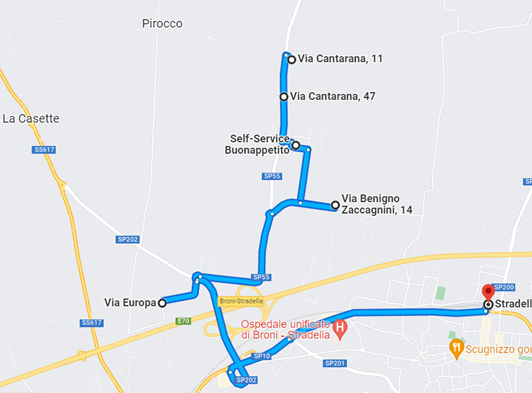
\includegraphics[width=0.7\textwidth]{Images/Scheduling/Path.png}
    \caption{Path from Business Park to Stradella FS}
    \label{fig:path}
\end{figure}




The additional stops, close to access point of the Business Park, will be:
\begin{itemize}
    \item Via Cantarana, 11 San Cipriniano Po
    \item Via Cantarana, 47 San Cipriniano Po
    \item Via dell'Industria, 1, 27049 Stradella PV
    \item Via Benigno Zaccagnini, 14 Stradella
    \item Via Europa, Broni
\end{itemize}


In the following pages the changes to the schedule time are reported. In figure \ref{fig:A1} and \ref{fig:A2} the changes due to the Scenario A (a creation of a tailor-made ride). In figure \ref{fig:B1} and \ref{fig:B2} the changes for scenario B (the modification of an existing ride).

The changes in yellow are consequences of the changes of the last stop of the bus. This has an effect also on the following rides because the bus is not in the same stop of the departure.

For the enter and exit at 6:00 and 22:00 we have only one scenario that consists in the creation of a new ride.

Regarding the changes for the entry at 08:30 in Figure \ref{fig:enter830} we can see the only changes the require the extension of ride 140021. For the exit at 17:30 the timetable is reported in Figure \ref{fig:exit1730}. This change does not impact on the other lines due to a greater headway. In the following section of this chapter a preliminary sizing of the new service is performed, quantifying the additional number of kilometers travelled, working hours and resources.

\newpage
\thispagestyle{empty}
\begin{landscape}
\begin{figure}[h]
    \centering
    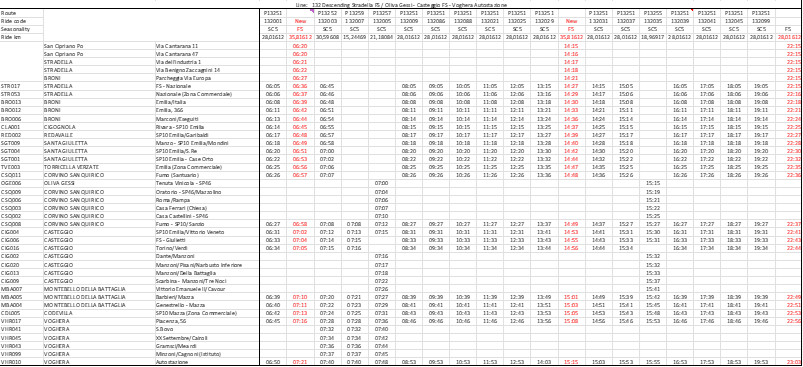
\includegraphics[width=1.4\textwidth]{Images/Scheduling/timetables/Scenario_A.png}
    \caption{Scenario A: Timetables for Enter at 6,14 and 22}
    \label{fig:A1}
\end{figure}
\end{landscape}


\newpage
\thispagestyle{empty}
\begin{landscape}
\begin{figure}[h]
    \centering
    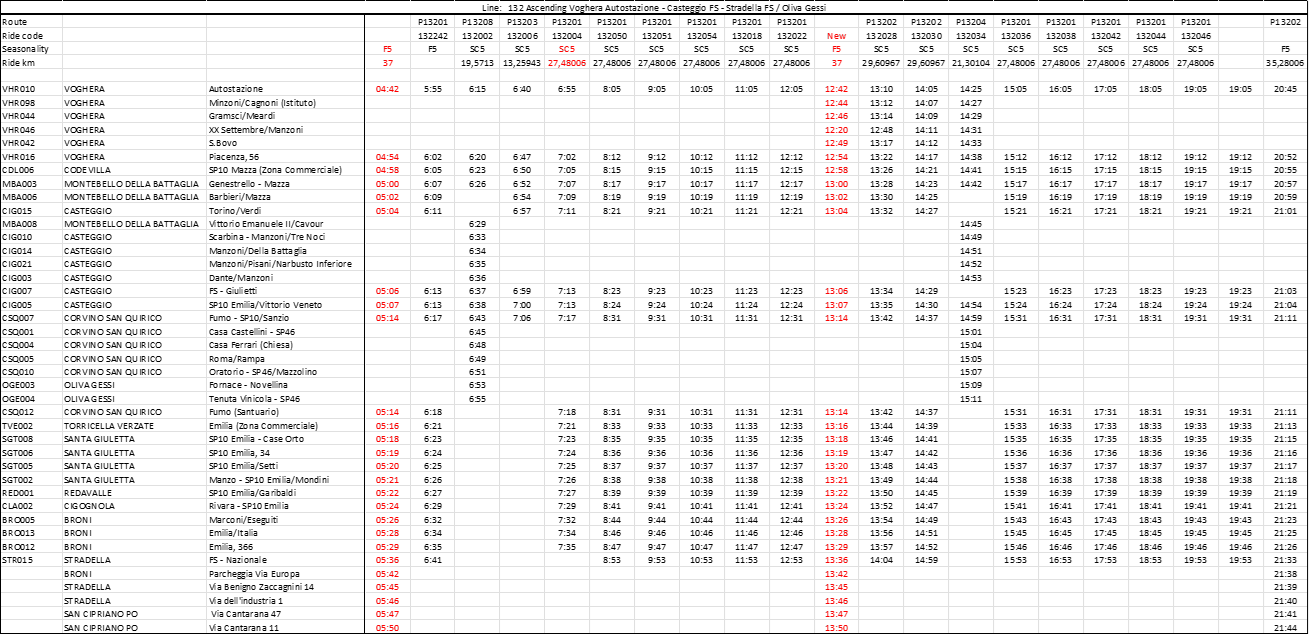
\includegraphics[width=1.4\textwidth]{Images/Scheduling/timetables/Scenario_A_2.png}
    \caption{Scenario A: Timetables for Exit at 6,14 and 22}
    \label{fig:A2}
\end{figure}
\end{landscape}
\newpage
\thispagestyle{empty}
\begin{landscape}
\begin{figure}[h]
    \centering
    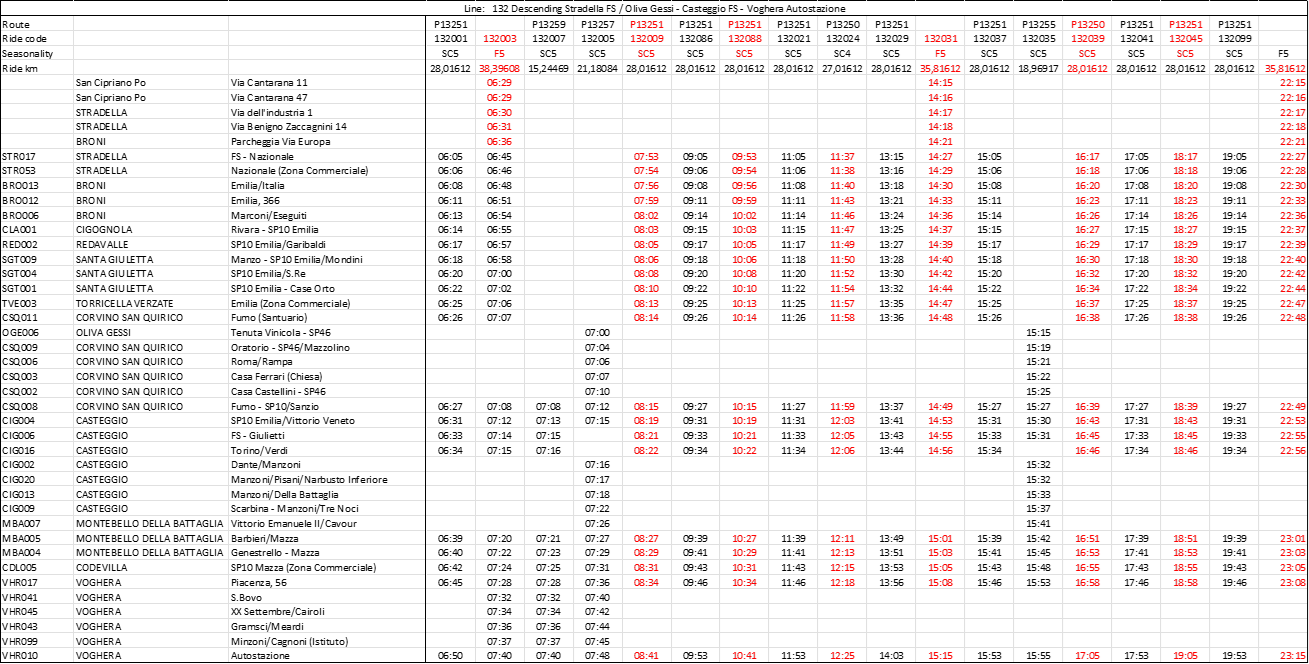
\includegraphics[width=1.4\textwidth]{Images/Scheduling/timetables/Scenario_B.png}
    \caption{Scenario B: Timetables for enter at 6,14 and 22}
    \label{fig:B1}
\end{figure}
\end{landscape}
\newpage
\thispagestyle{empty}
\begin{landscape}
\begin{figure}[h]
    \centering
    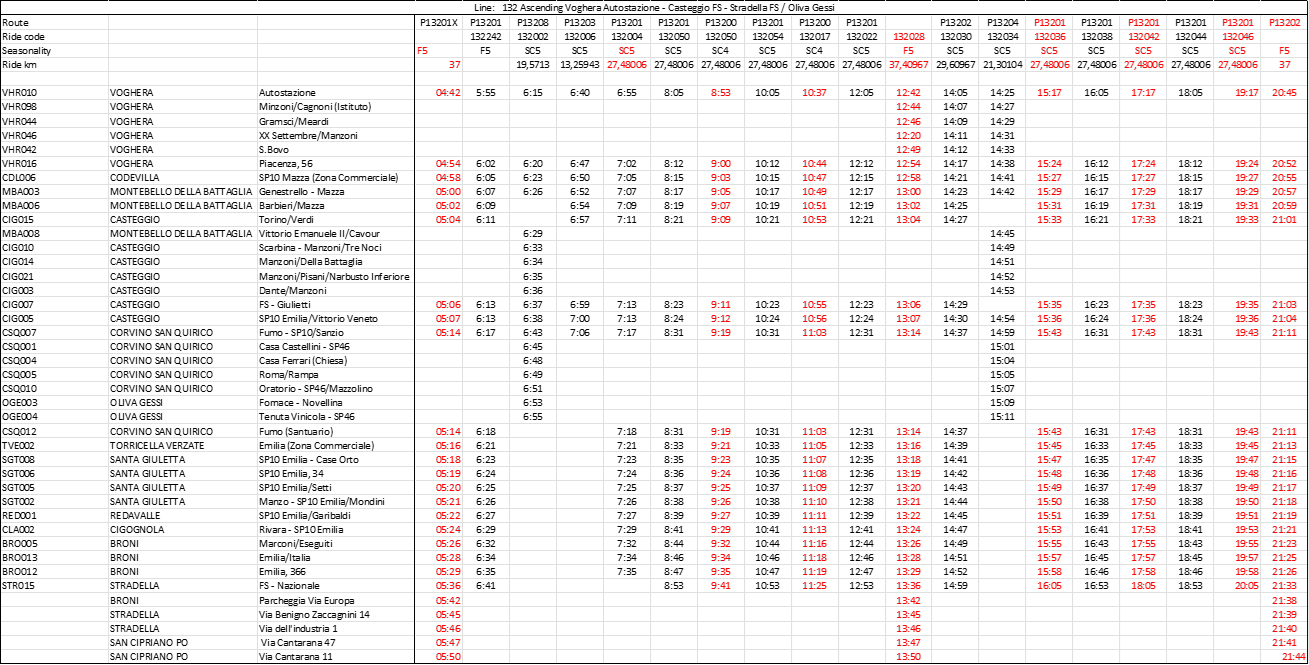
\includegraphics[width=1.4\textwidth]{Images/Scheduling/timetables/Scenario_B_2.png}
    \caption{Scenario B: Timetables for exit at 6,14 and 22}
    \label{fig:B2}
\end{figure}
\end{landscape}
\newpage
\thispagestyle{empty}
\begin{figure}[h]
    \centering
    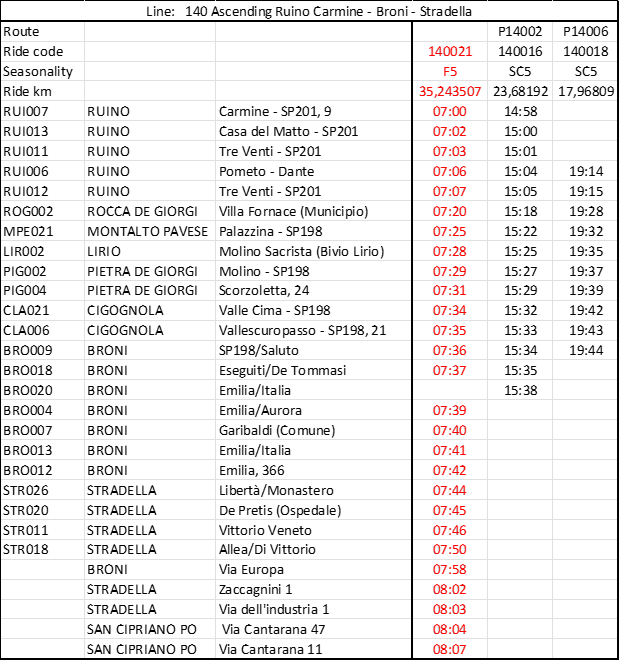
\includegraphics[width=1\textwidth]{Images/Scheduling/timetables/enter_8_30.png}
    \caption{Timetables for enter at 8:30}
    \label{fig:enter830}
\end{figure}
\newpage
\thispagestyle{empty}
\begin{figure}[h!]
    \centering
    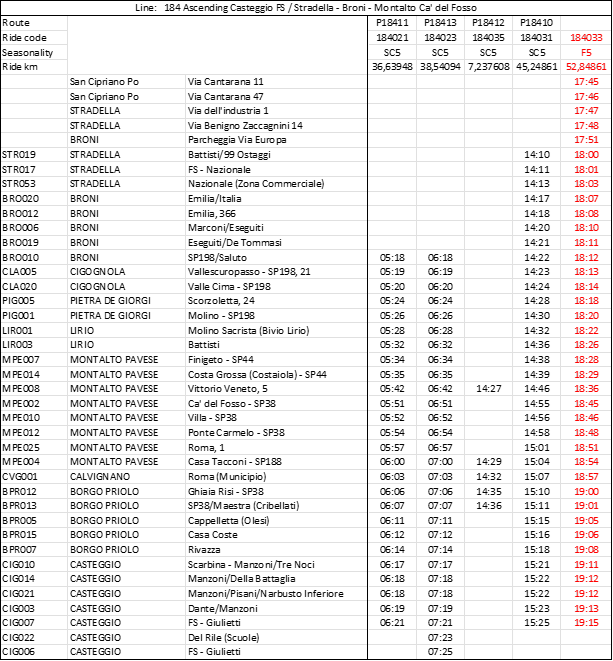
\includegraphics[width=1\textwidth]{Images/Scheduling/timetables/Exit_17_30.png}
    \caption{Timetables for enter at 17:30}
    \label{fig:exit1730}
\end{figure}
\newpage
\newpage

\section{Sizing}
This evaluation will be dependent on the different actions required to fit the new scheduling. In this case two options are available: the creation of a new ride from scratch or, if minor changes are suitable, a slight advance or delay of an existing one. Since the information of drivers and bus shift is not sufficiently detailed so as to integrate changes with the existing one, the assumption was that each new ride requires a dedicated driver and bus.
In detail, the rides requiring an additional bus and drivers are 
\paragraph{Start of shift 6:00}

The solution adopted for this shift is common for both the scenarios: the introduction of an additional ride. This requires an additional bus and driver for 37 km and 68 minutes.
\paragraph{End of shift 6:00}

According to the scheduling, the new ride is performed exploiting the presence of bus and driver in the Business Park for the start of shift 6:00. 
\begin{description}
    \item[Scenario A]: a tailor-made ride is created, with all the consequences implied in terms of kilometers and resources.
    \item[Scenario B]: the modification of an existing ride, extending its path and advancing the schedule.
\end{description}

\paragraph{Start of shift 8:30}

The solution adopted for this shift is common for both the scenarios: the modification of an existing ride extending its path till the Business Park for 4.9 km and 17 minutes, without the need of a new bus and driver.
\paragraph{Start and end of shift 14:00}

The resulting scenarios, for both arrival and departure, follow the same logic presented for the end of shift 6:00. Scenario A consists in the implementation of a completely new ride, while Scenario B exploits existing rides modified in their paths and routes in order to serve the Business Park.

\paragraph{End of shift 17:30}

The solution adopted for this shift is common for both the scenarios: the modification of an existing ride extending its path from the Business Park for 7.6 km and 15 minutes, without the need of a new bus and driver.
\paragraph{Start and end of shift 22:00}

The solutions adopted for both arrival and departure are the implementation of two new rides. Anyway, these two rides share the same bus and driver.

% Please add the following required packages to your document preamble:
% \usepackage{multirow}
% \usepackage[table,xcdraw]{xcolor}
% If you use beamer only pass "xcolor=table" option, i.e. \documentclass[xcolor=table]{beamer}
\begin{table}[h]
\centering
\begin{tabular}{|ll|l|c|c|l|l|l|}
\hline
\rowcolor{bluepoli!40}
\multicolumn{1}{|c|}{\textbf{Shift}} & \multicolumn{1}{c|}{\textbf{\begin{tabular}[c]{@{}c@{}}To/From \\ BP\end{tabular}}} & \multicolumn{1}{c|}{\textbf{km}} & \textbf{Drivers}         & \textbf{Buses}           & \multicolumn{1}{c|}{\textbf{\begin{tabular}[c]{@{}c@{}}time \\ {[}min{]}\end{tabular}}} & \multicolumn{1}{c|}{\textbf{km/year}} & \multicolumn{1}{c|}{\textbf{h/year}} \\ \hline
\multicolumn{1}{|l|}{06:00}          & To                                                                                  & 37                               &                          &                          & 68                                                                                      & 9398                                  & 269                                  \\ \cline{1-3} \cline{6-8} 
\multicolumn{1}{|l|}{06:00}          & From                                                                                & 36                               & \multirow{-2}{*}{1}      & \multirow{-2}{*}{1}      & 61                                                                                      & 9144                                  & 261                                  \\ \hline
\multicolumn{1}{|l|}{08:30}          & To                                                                                  & 4,9                              & 0                        & 0                        & 17                                                                                      & 3409,2                                & 97                                   \\ \hline
\multicolumn{1}{|l|}{14:00}          & To                                                                                  & 37                               &                          &                          & 68                                                                                      & 9398                                  & 269                                  \\ \cline{1-3} \cline{6-8} 
\multicolumn{1}{|l|}{14:00}          & From                                                                                & 36                               & \multirow{-2}{*}{1}      & \multirow{-2}{*}{1}      & 60                                                                                      & 9144                                  & 261                                  \\ \hline
\multicolumn{1}{|l|}{17:30}          & From                                                                                & 7,6                              & 0                        & 0                        & 15                                                                                      & 5485,4                                & 157                                  \\ \hline
\multicolumn{1}{|l|}{22:00}          & To                                                                                  & 35                               &                          &                          & 55                                                                                      & 8890                                  & 254                                  \\ \cline{1-3} \cline{6-8} 
\multicolumn{1}{|l|}{22:00}          & From                                                                                & 36                               & \multirow{-2}{*}{1}      & \multirow{-2}{*}{1}      & 60                                                                                      & 9144                                  & 261                                  \\ \hline
\multicolumn{2}{|l|}{sum}                                                                                                  & 229.5                            & 3 & 3 & 404                                                                                     & 64012,6                               & 1829                                 \\ \hline
\end{tabular}
\caption{Scenario A: additional resources}
\label{tab:addresA}
\end{table}

% Please add the following required packages to your document preamble:
% \usepackage{multirow}
\begin{table}[h]
\centering
\begin{tabular}{|ll|l|l|l|l|l|l|}
\hline
\rowcolor{bluepoli!40}
\multicolumn{1}{|c|}{\textbf{Shift}} & \multicolumn{1}{c|}{\textbf{\begin{tabular}[c]{@{}c@{}}To/From \\ BP\end{tabular}}} & \multicolumn{1}{c|}{\textbf{Km}} & \multicolumn{1}{c|}{\textbf{Drivers}} & \multicolumn{1}{c|}{\textbf{Buses}} & \multicolumn{1}{c|}{\textbf{\begin{tabular}[c]{@{}c@{}}time \\ {[}min{]}\end{tabular}}} & \multicolumn{1}{c|}{\textbf{km/year}} & \multicolumn{1}{c|}{\textbf{h/year}} \\ \hline
\multicolumn{1}{|l|}{06:00}          & To                  & 37          & 1                  & 1                  & 68                      & 9398             & 269                 \\ \hline
\multicolumn{1}{|l|}{06:00}          & From                & 7.8         & 0                  & 0                  & 16                      & 3614,6           & 103                 \\ \hline
\multicolumn{1}{|l|}{08:30}          & To                  & 4.9         & 0                  & 0                  & 17                      & 3409,2           & 97                  \\ \hline
\multicolumn{1}{|l|}{14:00}          & To                  & 7.8         & 0                  & 0                  & 14                      & 11514            & 329                 \\ \hline
\multicolumn{1}{|l|}{14:00}          & From                & 7.8         & 0                  & 0                  & 12                      & 4300,4           & 123                 \\ \hline
\multicolumn{1}{|l|}{17:30}          & From                & 7.6         & 0                  & 0                  & 15                      & 11260            & 322                 \\ \hline
\multicolumn{1}{|l|}{22:00}          & To                  & 35          & \multirow{2}{*}{1} & \multirow{2}{*}{1} & 55                      & 8890             & 254                 \\ \cline{1-3} \cline{6-8} 
\multicolumn{1}{|l|}{22:00}          & From                & 36          &                    &                    & 60                      & 9144             & 261                 \\ \hline
\multicolumn{2}{|l|}{sum}                                  & 143.9       & 2                  & 2                  & 257                     & 61530,2          & 1758                \\ \hline
\end{tabular}
\caption{Scenario B: Additional resource}
\label{tab:addresB}
\end{table}

With the scenario B (changes of the rides) solution about 2500 km/year and 71 hours/year are saved.

Some remarks on table \ref{tab:addresA} and \ref{tab:addresB}:
\begin{enumerate}
    \item Since the working hours of a driver is generally 6 hours, probably it should be enough for Scenario A to add only two drivers ($404 min/(60 min/h \cdot 6 h/driver) = 1.12 drivers \approx 2 drivers$), while for Scenario B one driver is enough.
    \item Since the rides are not at the same time, probably only one bus should be enough for both the Scenarios
\end{enumerate}
\chapter{Financial Assessment}
In this part an analysis of the economic performances of the service proposals is presented. The analysis follows the two scenarios:
•	A: characterized by the implementation of new rides from scratch;
•	B: defined by modification of the actual lines.
The objective of this part is to access the scenario that, a parity of level of service for the customer and general assumptions, is the most financially profitable and sustainable.
The initial part regarding the Fare Revenues analysis is common for both the scenario. Instead, the economic performance of the two scenarios will be studied separately.


\paragraph{Economic Analysis assumptions}
The provided assumption used to perform this analysis are reported for reference in the table \ref{tab:specificcostbus} and regards the specific cost of a bus service. 

% Please add the following required packages to your document preamble:
% \usepackage[table,xcdraw]{xcolor}
% If you use beamer only pass "xcolor=table" option, i.e. \documentclass[xcolor=table]{beamer}
% \usepackage{lscape}

\begin{table}[H]
\centering
\begin{tabular}{lll}
\hline
\rowcolor{bluepoli!40}
\multicolumn{1}{|c|}{{\color[HTML]{333333} \textbf{Bus operation related cost}}} & \multicolumn{1}{c|}{{\color[HTML]{333333} \textbf{Local   currency}}} & \multicolumn{1}{c|}{{\color[HTML]{333333} \textbf{12   m bus}}} \\ \hline
\multicolumn{1}{|l|}{{\color[HTML]{333333} Fuel price}}                          & \multicolumn{1}{l|}{{\color[HTML]{333333} €/Litre}}                   & \multicolumn{1}{l|}{{\color[HTML]{333333} 1.20}}                \\ \hline
\multicolumn{1}{|l|}{{\color[HTML]{333333} Fuel Consumption}}                    & \multicolumn{1}{l|}{{\color[HTML]{333333} Km/Litre}}                  & \multicolumn{1}{l|}{{\color[HTML]{333333} 2.50}}                \\ \hline
\multicolumn{1}{|l|}{{\color[HTML]{333333} Maintenance cost per year}}           & \multicolumn{1}{l|}{{\color[HTML]{333333} €/Km}}                      & \multicolumn{1}{l|}{{\color[HTML]{333333} 0.25}}                \\ \hline
\multicolumn{1}{|l|}{{\color[HTML]{333333} Mileage per year}}                    & \multicolumn{1}{l|}{{\color[HTML]{333333} Km}}                        & \multicolumn{1}{l|}{{\color[HTML]{333333} 50,000}}              \\ \hline
\multicolumn{1}{|l|}{{\color[HTML]{333333} Capital expenditure per bus}}         & \multicolumn{1}{l|}{{\color[HTML]{333333} €}}                         & \multicolumn{1}{l|}{{\color[HTML]{333333} 200,000}}             \\ \hline
\multicolumn{1}{|l|}{{\color[HTML]{333333} Years in operation}}                  & \multicolumn{1}{l|}{{\color[HTML]{333333} \#}}                        & \multicolumn{1}{l|}{{\color[HTML]{333333} 15}}                  \\ \hline
\multicolumn{1}{|l|}{{\color[HTML]{333333} Amortization index}}                  & \multicolumn{1}{l|}{{\color[HTML]{333333} \#}}                        & \multicolumn{1}{l|}{{\color[HTML]{333333} 6.7\%}}               \\ \hline
{\color[HTML]{333333} }                                                          & {\color[HTML]{333333} }                                               & {\color[HTML]{333333} }                                         \\ \hline
\rowcolor{bluepoli!40}\multicolumn{1}{|c|}{{\color[HTML]{333333} \textbf{Other Costs}}}                & \multicolumn{1}{c|}{{\color[HTML]{333333} \textbf{Local   currency}}} & \multicolumn{1}{l|}{{\color[HTML]{333333} }}                    \\ \hline
\multicolumn{1}{|l|}{{\color[HTML]{333333} Driver cost per year STD}}            & \multicolumn{1}{l|}{{\color[HTML]{333333} €}}                         & \multicolumn{1}{l|}{{\color[HTML]{333333} 35,000}}              \\ \hline
\multicolumn{1}{|l|}{{\color[HTML]{333333} workdays}}                            & \multicolumn{1}{l|}{{\color[HTML]{333333} }}                          & \multicolumn{1}{l|}{{\color[HTML]{333333} 250}}                 \\ \hline
\multicolumn{1}{|l|}{{\color[HTML]{333333} hours per year STD}}                  & \multicolumn{1}{l|}{{\color[HTML]{333333} }}                          & \multicolumn{1}{l|}{{\color[HTML]{333333} 1,800}}               \\ \hline
\multicolumn{1}{|l|}{{\color[HTML]{333333} Insurance per bus}}                   & \multicolumn{1}{l|}{{\color[HTML]{333333} €/bus}}                     & \multicolumn{1}{l|}{{\color[HTML]{333333} 2,000}}               \\ \hline
\multicolumn{1}{|l|}{{\color[HTML]{333333} Selling expenses}}                    & \multicolumn{1}{l|}{{\color[HTML]{333333} }}                          & \multicolumn{1}{l|}{{\color[HTML]{333333} 2\%}}                 \\ \hline
\multicolumn{1}{|l|}{{\color[HTML]{333333} Annual budget marketing expenses}}    & \multicolumn{1}{l|}{{\color[HTML]{333333} }}                          & \multicolumn{1}{l|}{{\color[HTML]{333333} 10,000}}              \\ \hline
\multicolumn{1}{|l|}{{\color[HTML]{333333} Tax}}                                 & \multicolumn{1}{l|}{{\color[HTML]{333333} }}                          & \multicolumn{1}{l|}{{\color[HTML]{333333} 27.9\%}}              \\ \hline
\end{tabular}
\caption{Specific cost of a Bus Service}
\label{tab:specificcostbus}
\end{table}% tabella


\section{Fare revenues}
To select the cost, a weighted average between the distance of the proposed service has been made: a weight of 80\% has been added to category 8 (to address the amount of workers arriving from Voghera); a weight of 20\% to category 3 (to address the workers arriving from Stradella and Broni). So, the resultant ticket category is 7.

The starting point of the fare revenue analyses has been the definition of its value on monthly base by the income from travel documents sale. This value is strongly correlated not simply with the number of tickets sold, but even more by the typology of the document due to the subscription discount factor.
\begin{table}[H]
\centering
\begin{tabular}{|l|l|l|l|l|}
\hline
\rowcolor{bluepoli!40}
\multicolumn{1}{|c|}{\textbf{\begin{tabular}[c]{@{}c@{}}Travel \\ Document \\ Typology\end{tabular}}} & \multicolumn{1}{c|}{\textbf{Cost}} & \multicolumn{1}{c|}{\textbf{\begin{tabular}[c]{@{}c@{}}\# journey \\ per ticket\end{tabular}}} & \multicolumn{1}{c|}{\textbf{\begin{tabular}[c]{@{}c@{}}Cost \\ of \\ single travel\end{tabular}}} & \multicolumn{1}{c|}{\textbf{\begin{tabular}[c]{@{}c@{}}Discount \\ factor\end{tabular}}} \\ \hline
Single ticket                                                                                         & 3.7                                & 1                                                                                              & 3.70                                                                                              & 0\%                                                                                      \\ \hline
10 Journey ticket                                                                                     & 34.5                               & 10                                                                                             & 3.45                                                                                              & 7\%                                                                                      \\ \hline
Weekly ticket                                                                                         & 24.5                               & 12                                                                                             & 2.04                                                                                              & 45\%                                                                                     \\ \hline
Monthly ticket                                                                                        & 86                                 & 48                                                                                             & 1.79                                                                                              & 52\%                                                                                     \\ \hline
Annual ticket                                                                                         & 830                                & 528                                                                                            & 1.57                                                                                              & 58\%                                                                                     \\ \hline
\end{tabular}
\caption{Tickets cost}
\label{tab:ticket}
\end{table}%tabella

In the following step, a possible composition of the travel documentation type is estimated. The first strong conceptual division of the analysis has been the differentiation between a high demand service and low demand ones, which is reflected into the general travel documentation typology composition.

\begin{figure}[h]
    \centering
    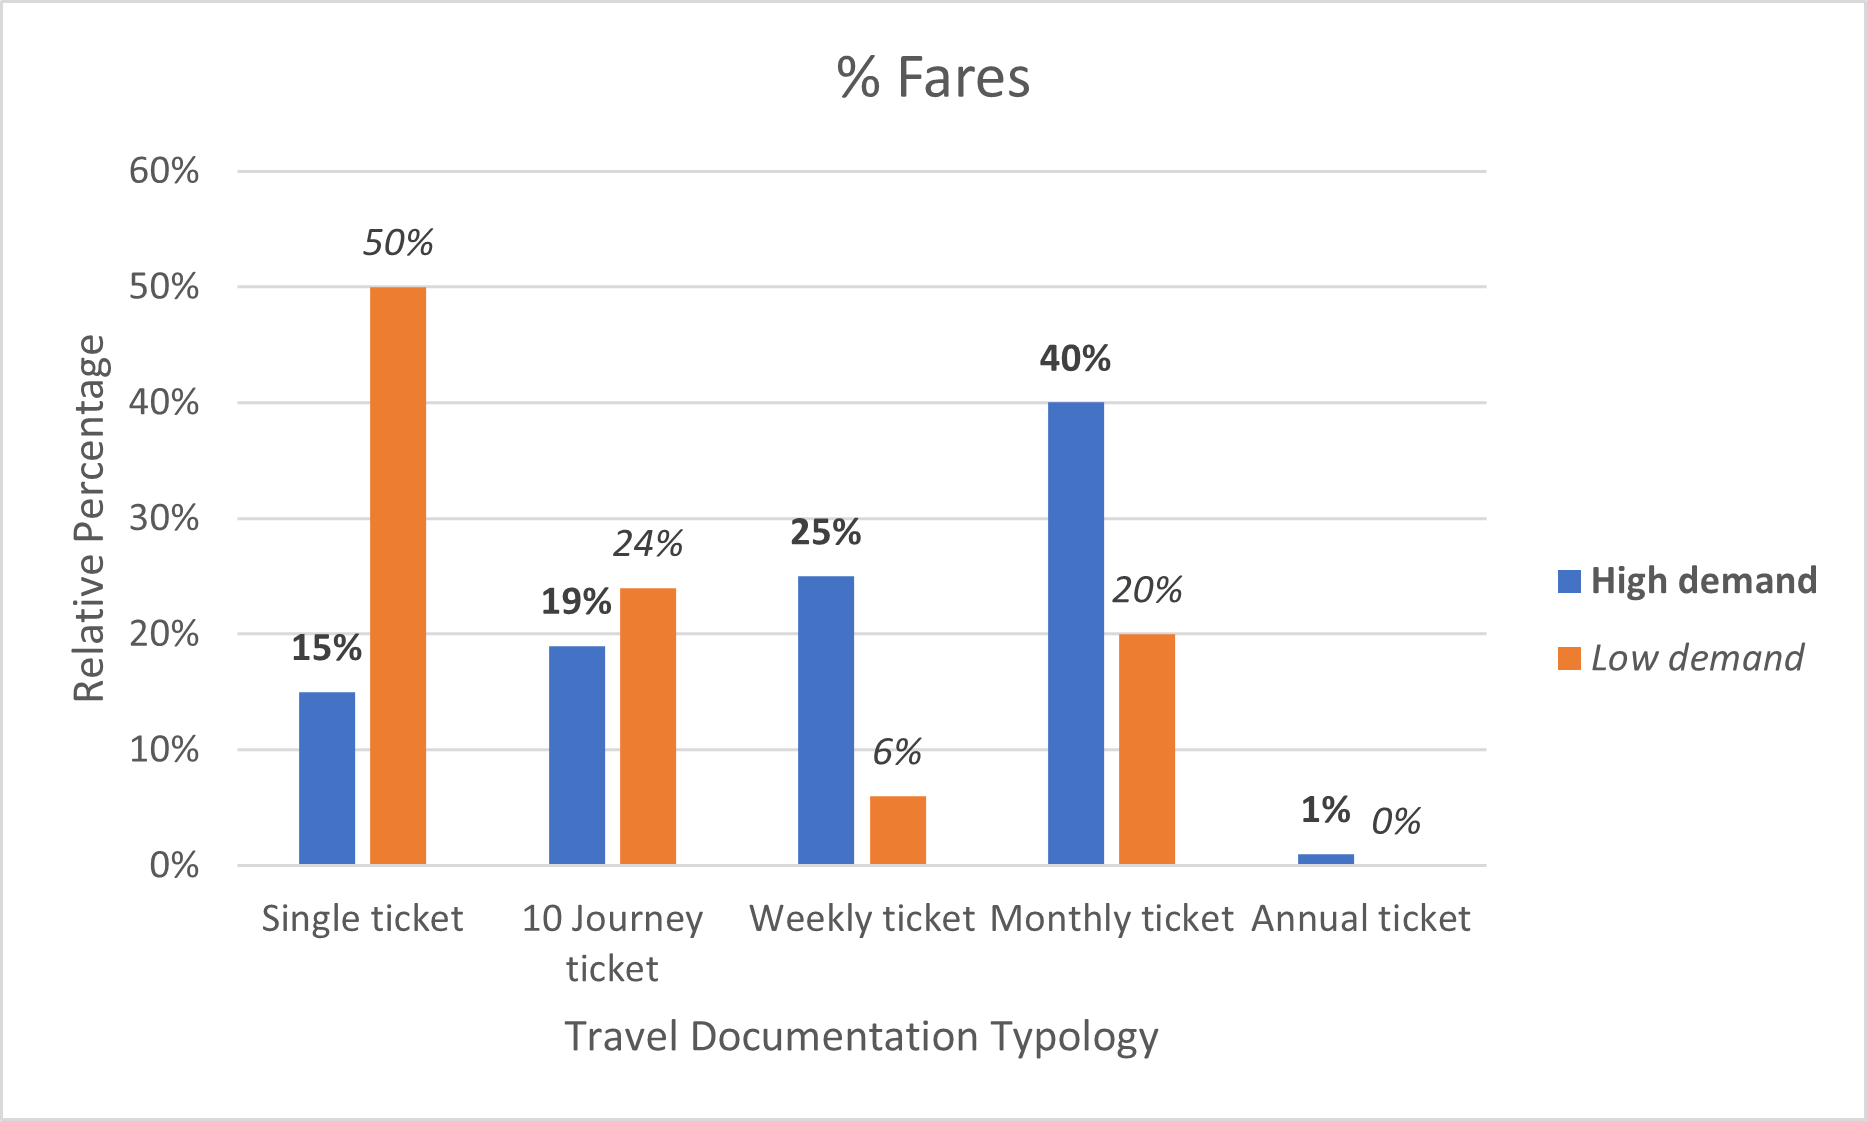
\includegraphics[width=0.7\textwidth]{Images/financial/fares.png}
    \caption{Fares percentage}
    \label{fig:fares_percentage}
\end{figure}
Considering the nature of the service under study, characterized by stable and a priori known demand, it can be easily clustered under the “High demand” service typology. This baseline feature is reflected in a travel documentation mix more oriented to subscription than single tickets.

The table \ref{tab:fare_distribution} and figure \ref{fig:fares_percentage2} represent the estimation of the travel documentation mix on the yearly base. This exercise has been performed to understand how the winter and summer working holiday period could be reflected in the customer choice.
\begin{figure}[h]
    \centering
    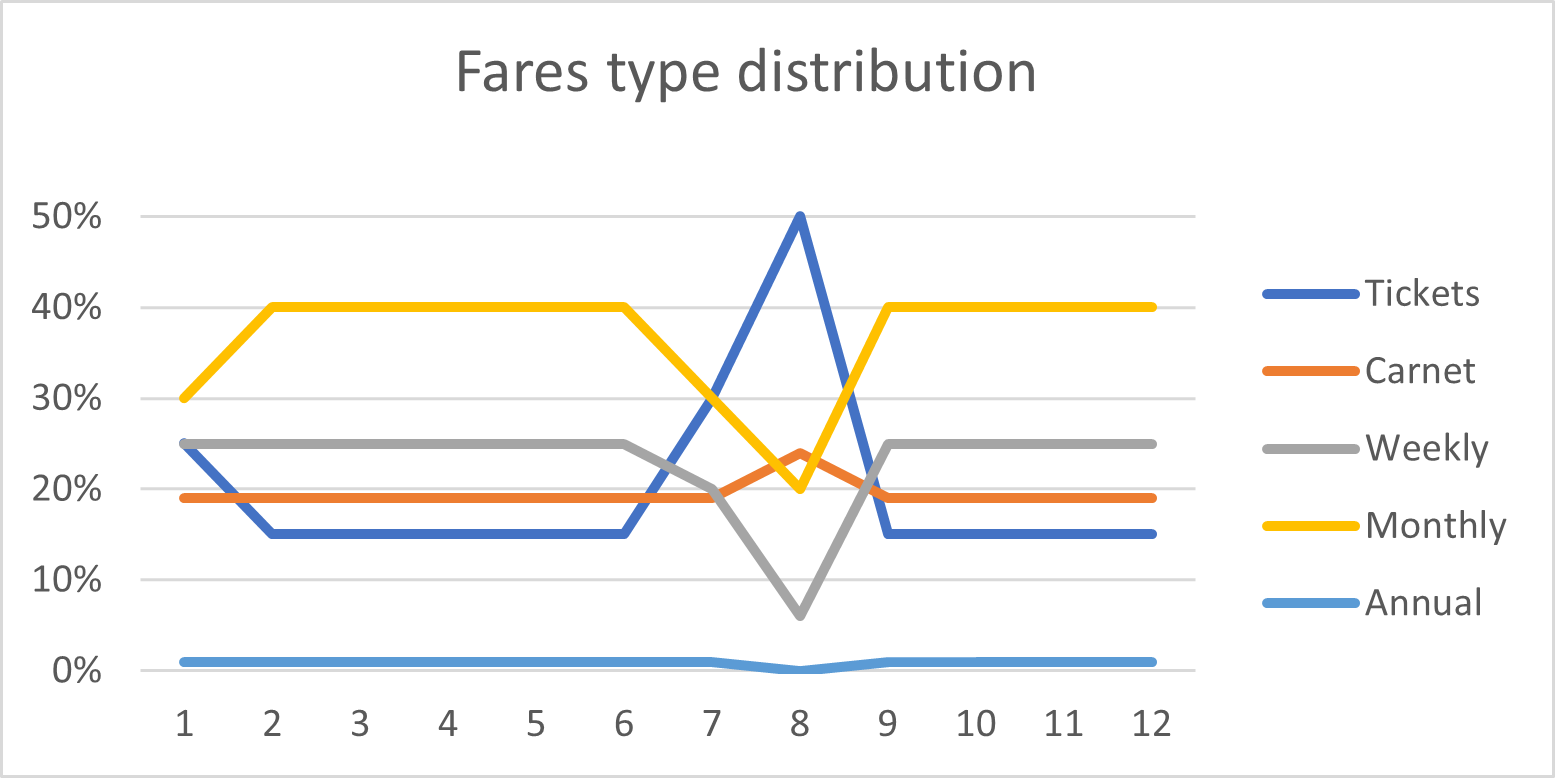
\includegraphics[width=0.7\textwidth]{Images/financial/fares_type_distribution.png}
    \caption{Fares percentage}
    \label{fig:fares_percentage2}
\end{figure}

% Please add the following required packages to your document preamble:
% \usepackage{multirow}
% \usepackage[table,xcdraw]{xcolor}
% If you use beamer only pass "xcolor=table" option, i.e. \documentclass[xcolor=table]{beamer}
\begin{table}[hp]
\centering
\begin{tabular}{|l|l|l|l|l|l|l|l|}
\hline
\rowcolor{bluepoli!40}
\multicolumn{1}{|c|}{\textbf{\begin{tabular}[c]{@{}c@{}}travel\\ documents\end{tabular}}} & \multicolumn{1}{c|}{{\color[HTML]{333333} \textbf{Year 1}}} & \multicolumn{1}{c|}{{\color[HTML]{333333} \textbf{Year 2}}} & \multicolumn{1}{c|}{{\color[HTML]{333333} \textbf{Year 3}}} & \multicolumn{1}{c|}{{\color[HTML]{333333} \textbf{Year 4}}} & \multicolumn{1}{c|}{{\color[HTML]{333333} \textbf{Year 5}}} & \multicolumn{1}{c|}{{\color[HTML]{333333} \textbf{Year 6}}} & \multicolumn{1}{c|}{\textbf{\begin{tabular}[c]{@{}c@{}}Yearly \\ variation {[}\%{]}\end{tabular}}} \\ \hline
Single ticket                                                                             & 19,584                                                      & 18,996                                                      & 18,427                                                      & 17,874                                                      & 17,338                                                      & 16,817                                                      & $-3\%$                                                                                             \\ \hline
10 Journey ticket                                                                         & 1,901                                                       & 1,863                                                       & 1,826                                                       & 1,789                                                       & 1,754                                                       & 1,719                                                       & $-2\%$                                                                                             \\ \hline
Weekly ticket                                                                             & 2,252                                                       & 2,253                                                       & 2,255                                                       & 2,256                                                       & 2,257                                                       & 2,258                                                       & $0\%$                                                                                              \\ \hline
Monthly ticket                                                                            & 898                                                         & 916                                                         & 934                                                         & 953                                                         & 972                                                         & 991                                                         & $2\%$                                                                                              \\ \hline
Annual ticket                                                                             & 22                                                          & 23                                                          & 23                                                          & 23                                                          & 23                                                          & 24                                                          & $1\%$                                                                                              \\ \hline
Annual journey                                                                            & 120,556                                                     & 120,583                                                     & 120,653                                                     & 120,766                                                     & 120,922                                                     & 121,120                                                     &                                                                                                    \\ \cline{1-7}
\begin{tabular}[c]{@{}l@{}}Fare \\ Reneues {[}€{]}\end{tabular}                           & 289,052                                                     & 287,326                                                     & 285,724                                                     & 284,243                                                     & 282,882                                                     & 281,639                                                     &                                                                                                    \\ \cline{1-7}
\begin{tabular}[c]{@{}l@{}}Fare \\ Reneues \\ variation {[}\%{]}\end{tabular}             & $0.0\%$                                                     & -0.6\%                                                      & $-1.2\%$                                                    & $-1.7\%$                                                    & $-2.1\%$                                                    & $-2.6\%$                                                    & \multirow{-3}{*}{}                                                                                 \\ \hline
\end{tabular}
\caption{Fare distribution output   }
\label{tab:fare_distribution}
\end{table}
Moving to the economical results of this travel documentation distribution mix, it is possible observing that the monthly ticket, that is around the 40\% of the total, generates the 60\% of the income.

\begin{figure}[h]
    \centering
    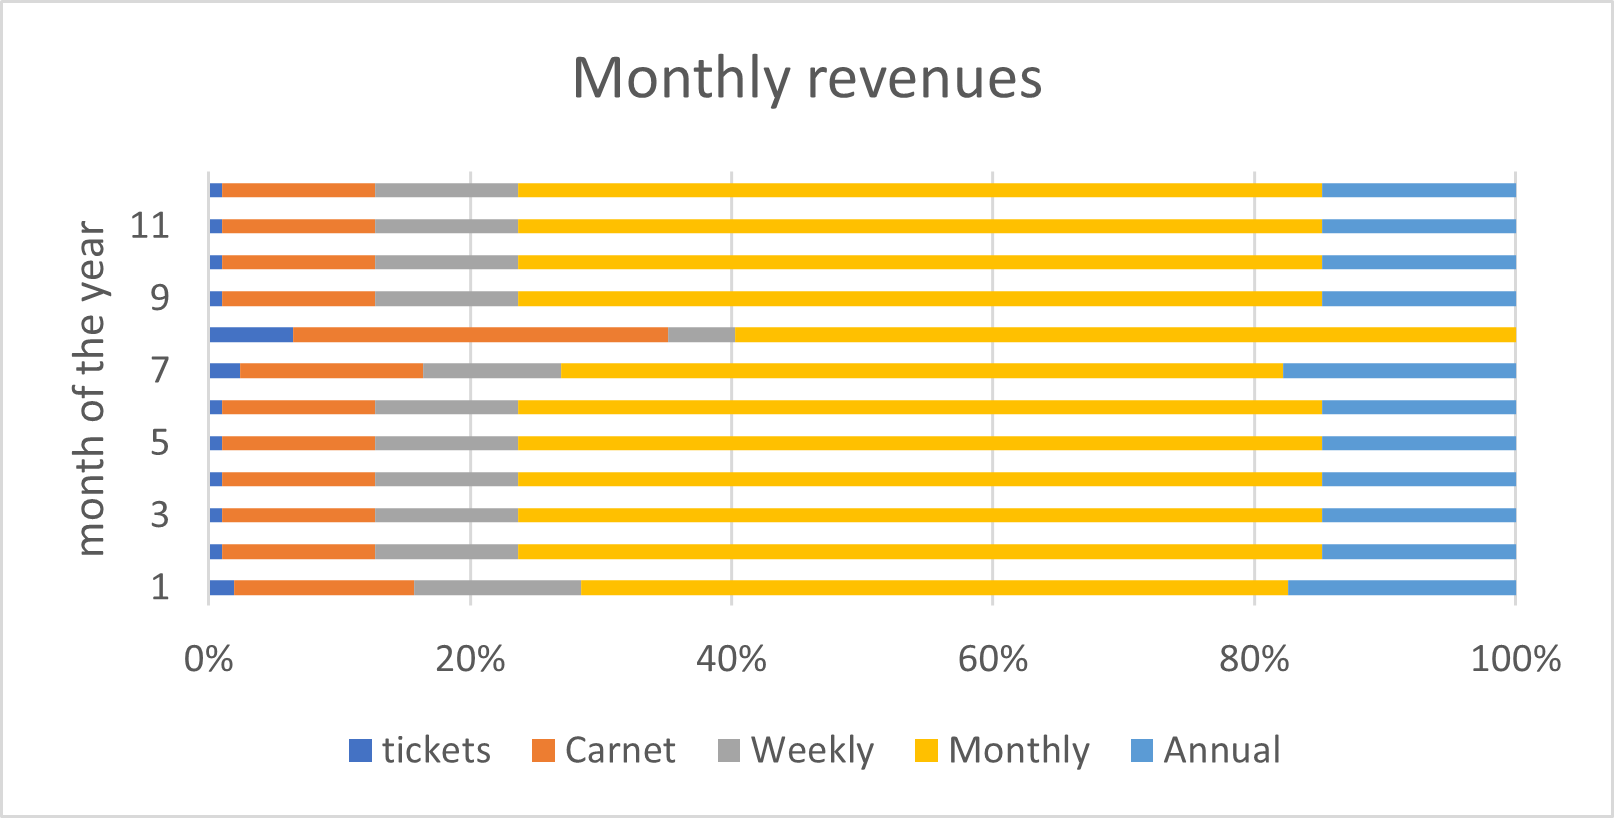
\includegraphics[width=0.7\textwidth]{Images/financial/monthly_revenues.png}
    \caption{Montlhy Revenues}
    \label{fig:monthly_revenues}
\end{figure}
To simulate the evolution of the customer behavior over the years under the “customer loyalty” concept, a progressive shift of the “ \% fares” from the short-term ticket type to the longer-term subscription is assumed and reported in the resuming table below.

Looking to the fare revenues results, the variation in the customer choice trend over the years leads to a constant erosion of the income due to the lower marginal value of the subscriptions. 

Given the positive financial results throughout the periods -showed in the following section-, this is not a negative phenomenon given the temporal profile nature of the subscription – comparable to a free interest tax loan – with respect to the single ticket ones. 

Finally, the figure \ref{fig:j_revenues} shows the relationship between journey performed, generated revenues and the ratio between ticket/subscription.

\begin{figure}[h]
    \centering
    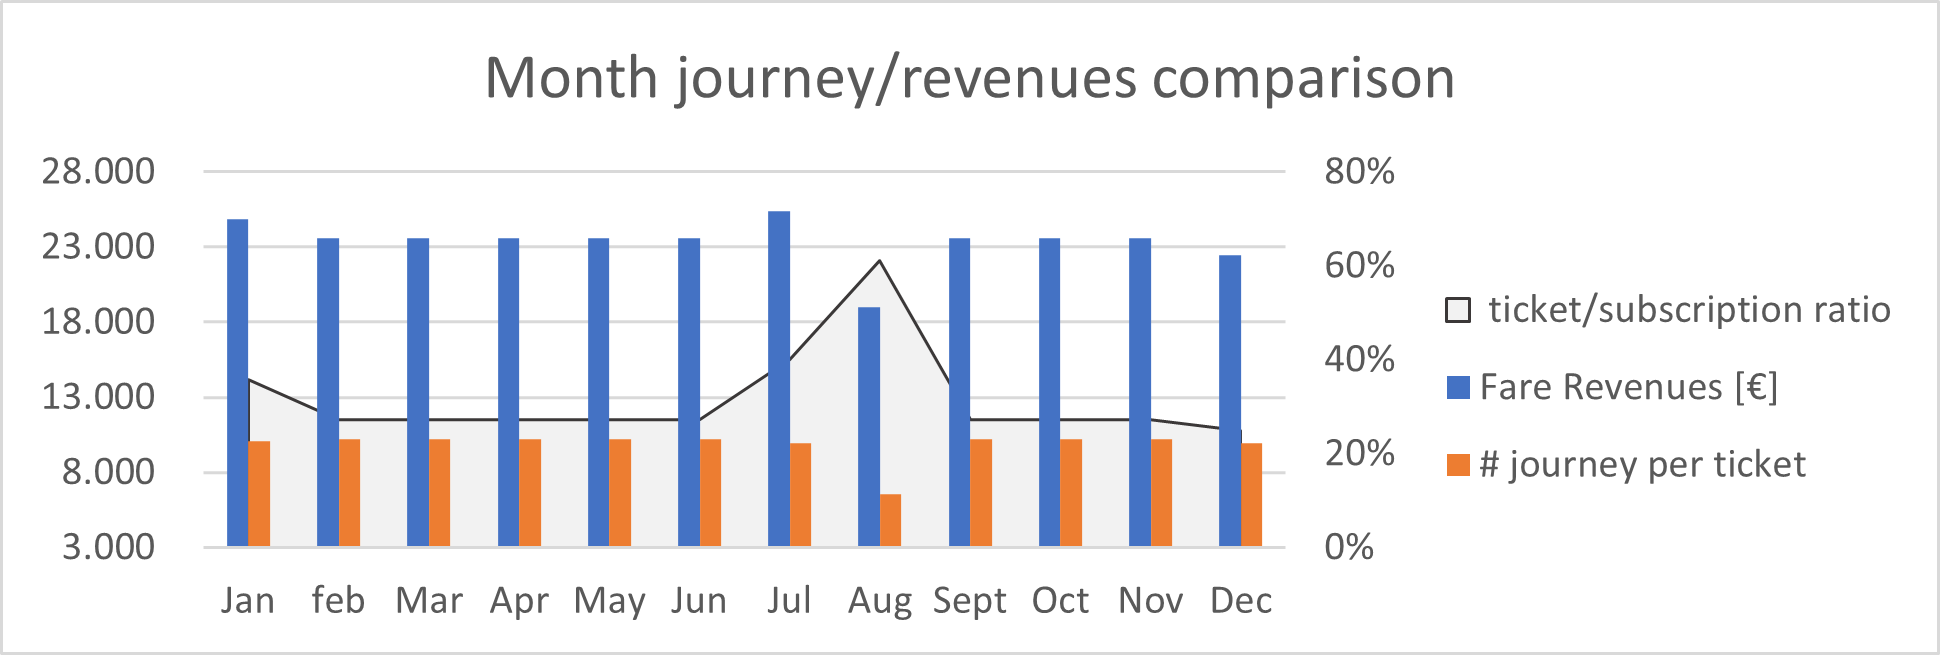
\includegraphics[width=0.7\textwidth]{Images/financial/journey_revenues.png}
    \caption{Journey Revenues}
    \label{fig:j_revenues}
\end{figure}

\section{Income statement}
Moving from the demand side to the offer one, the different economic performances of the two-service implementation scenario is analyzed. Their common feature are the distance between the depot and the service starting point (which accounts for 1.8 km) and the decision to avoid the usage of public subsidies, under the general idea to develop a self-sustainable business model.

\paragraph{scenario A}
Starting from the scenario A, it records an annual milage of 64 thousand of kilometers of which the 97\% in the economically productive “in service” state, and the remaining for the depo transfer. For more communicative data visualization, in figure \ref{fig:incstateA} are reported only major voices of the income statement.

\begin{figure}[h]
    \centering
    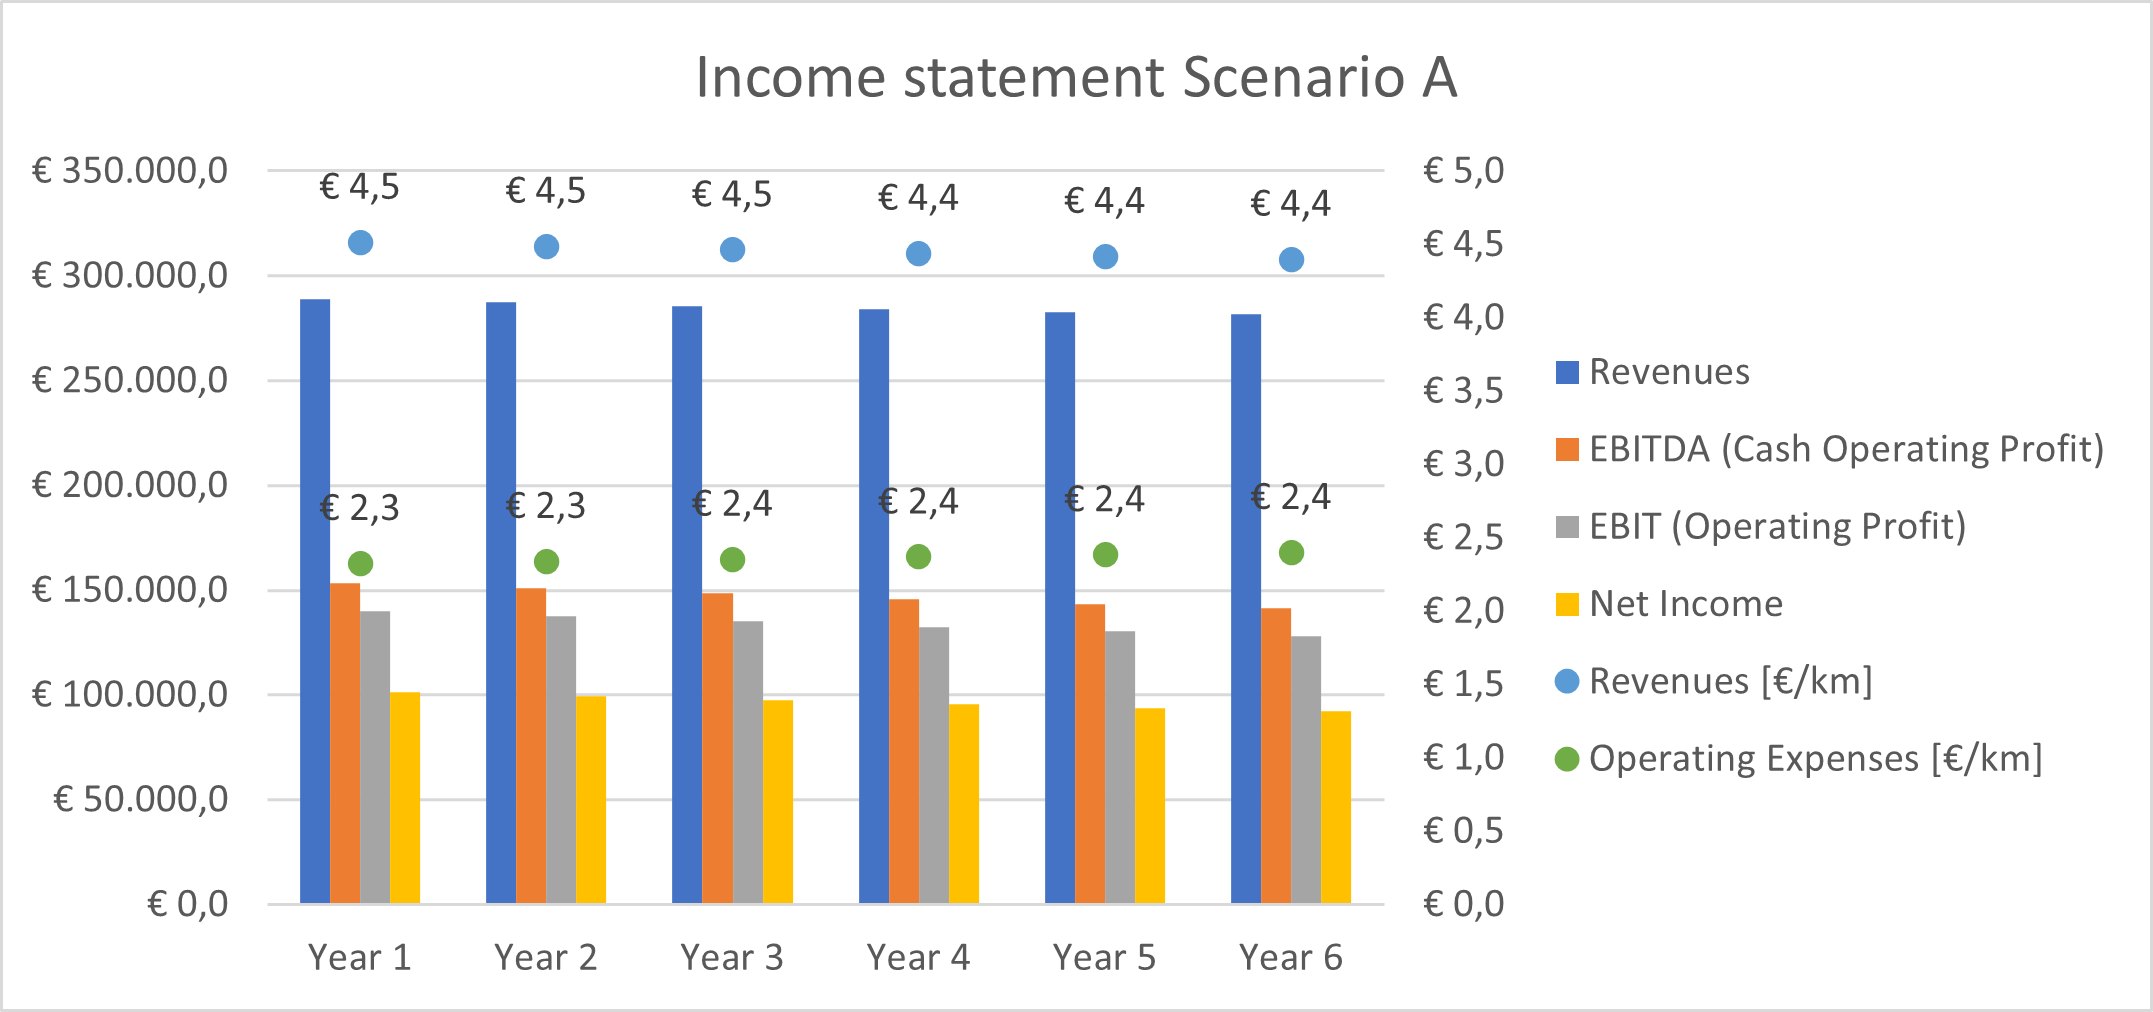
\includegraphics[width=0.7\textwidth]{Images/financial/income_statement_A.png}
    \caption{Scenario A: Income Statement}
    \label{fig:incstateA}
\end{figure}

Looking to the cost Structure, obtained by the “Cost of Goods and services” voice and showed in the pie chart below, it is noticed a slightly different composition respect to a traditional PTO cost structure, with an higher fuel cost incidence and a slightly less driver ones. 

\paragraph{scenario B}
Analyzing the second scenario, the B one, we have a small reduction in the annual performed milage (which accounts for 61.5 thousand annual kilometer, the 4\% less) with a consequent slightly higher incidence of the “Out of service” milage, which accounts for the 5\%. Nevertheless, despite these small variation, we almost have a coincidence in these previously values showing how the “hard” route deviation in the scenario B produce similar performances in the service implementation strategy with respect to the scenario A
The main Income statement voices related to this scenario are visualized in the \ref{fig:incstateB}.

\begin{figure}[h]
    \centering
    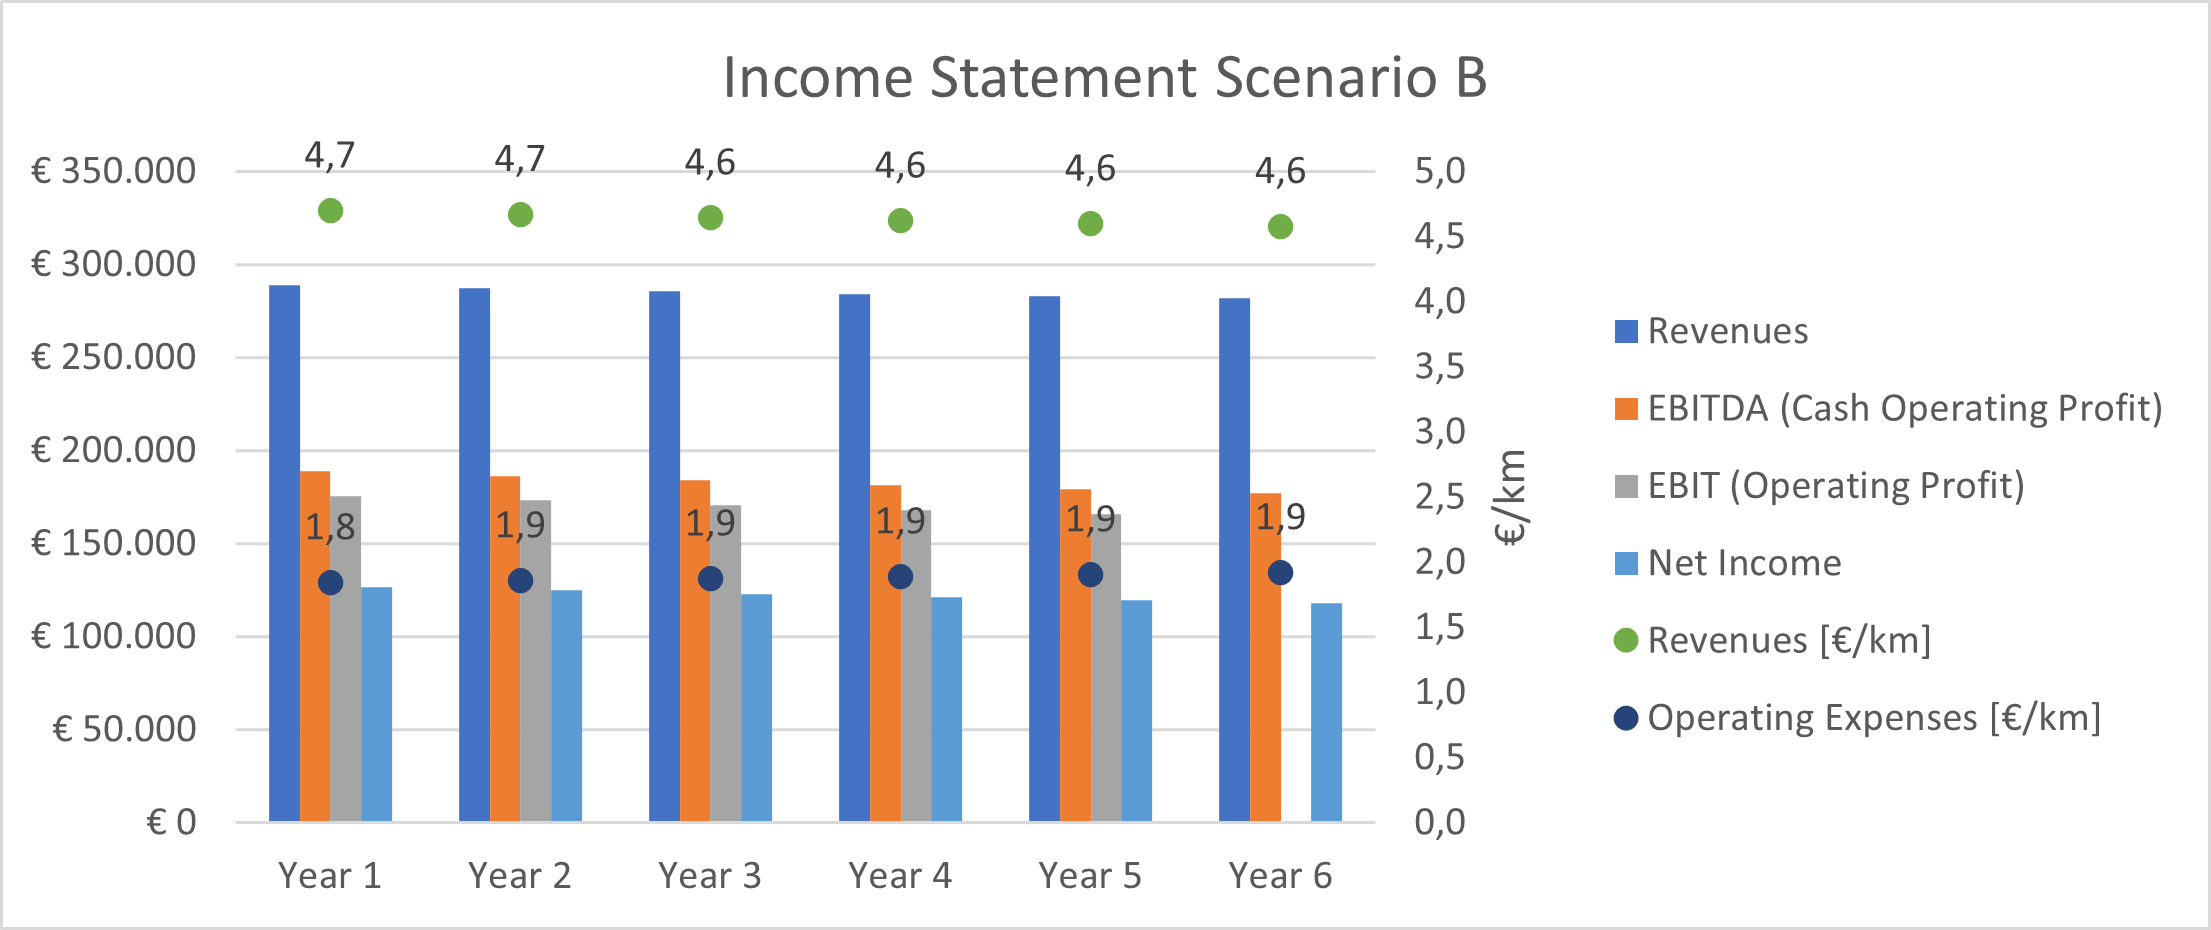
\includegraphics[width=0.7\textwidth]{Images/financial/income_statement_B.png}
    \caption{Scenario B: Income Statement}
    \label{fig:incstateB}
\end{figure}

\begin{figure}[h]
    \centering
    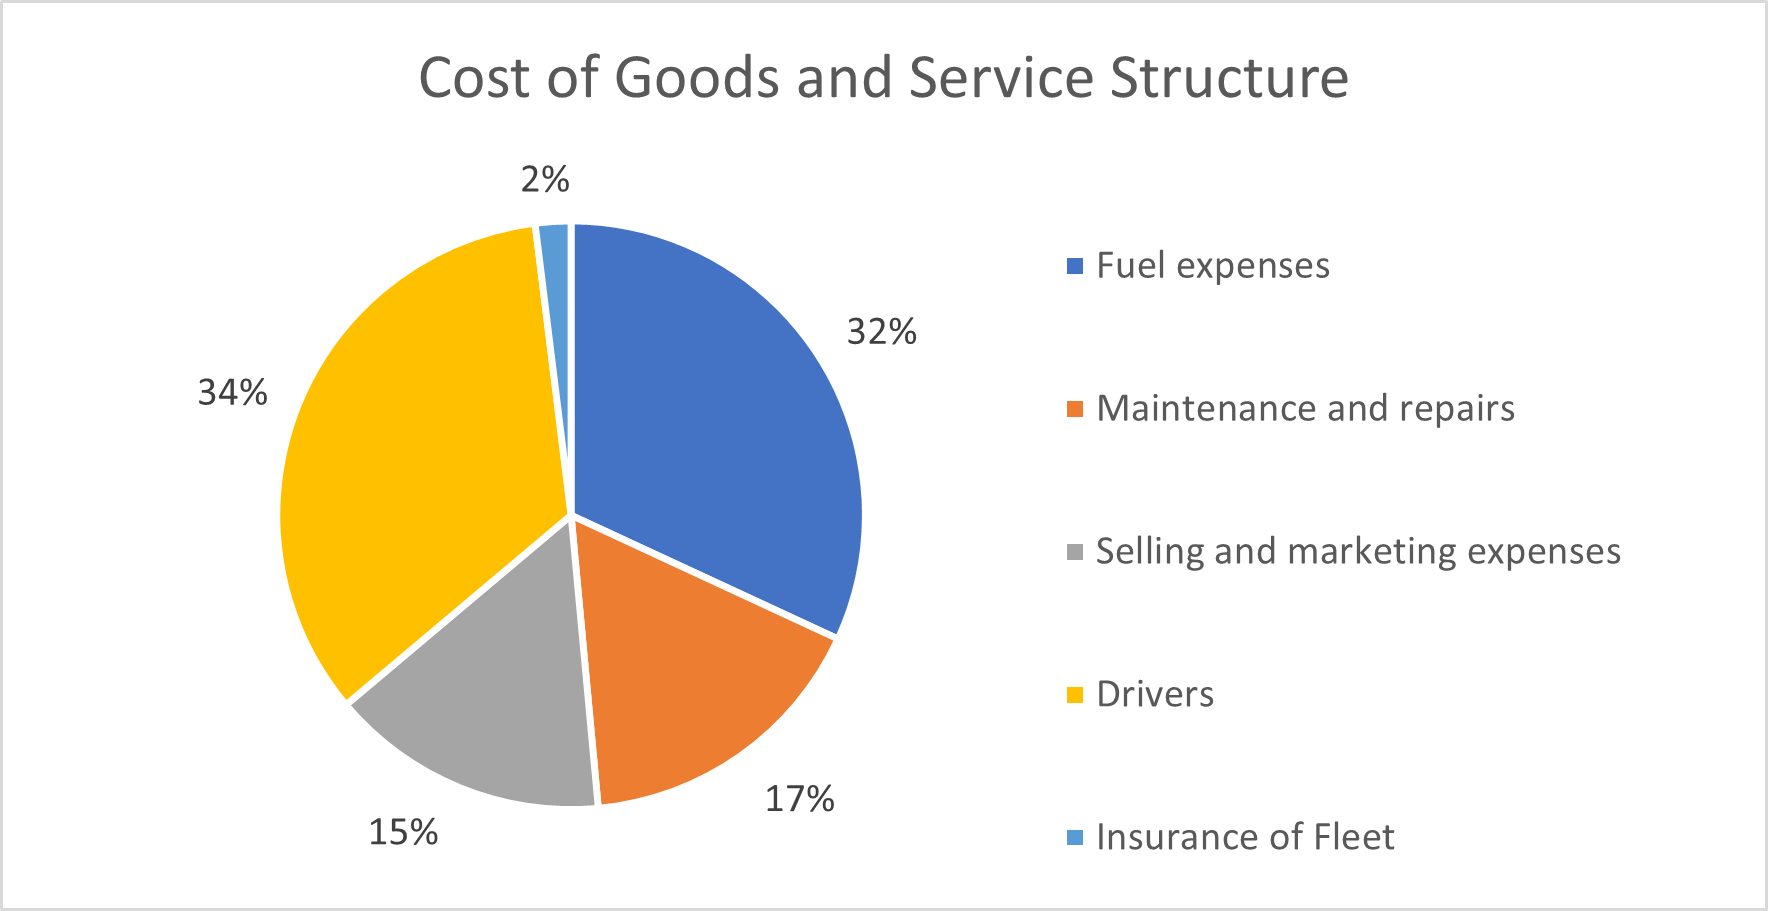
\includegraphics[width=0.7\textwidth]{Images/financial/Cost_of_Goods.png}
    \caption{Cost of Goods and Service Structure}
    \label{fig:costgoodsservice}
\end{figure}

\subsection{Income statement comparison}
Both the service scenarios scores more than acceptable economic performance all over the 6 studied year without the grants’ needs and without the effect of the progressively yearly revenues reduction.
The side-to-side comparison (reported in \ref{fig:income_statement_comparison}of the main income statement voices shows clearly how, from an economic perspective, the scenario B produce better economic performance. 

This phenomenon is simply due to the fewer operating cost of the B service (which perform less annual milage) and consequently by the higher ratio between revenues over distance – same revenue over a smaller distance. 

Consequently, given that the two scenarios produce the identical level of service for the customer, we agree to select the B scenario as best way for the company to implement the service in the most efficient way.

\begin{figure}[h]
    \centering
    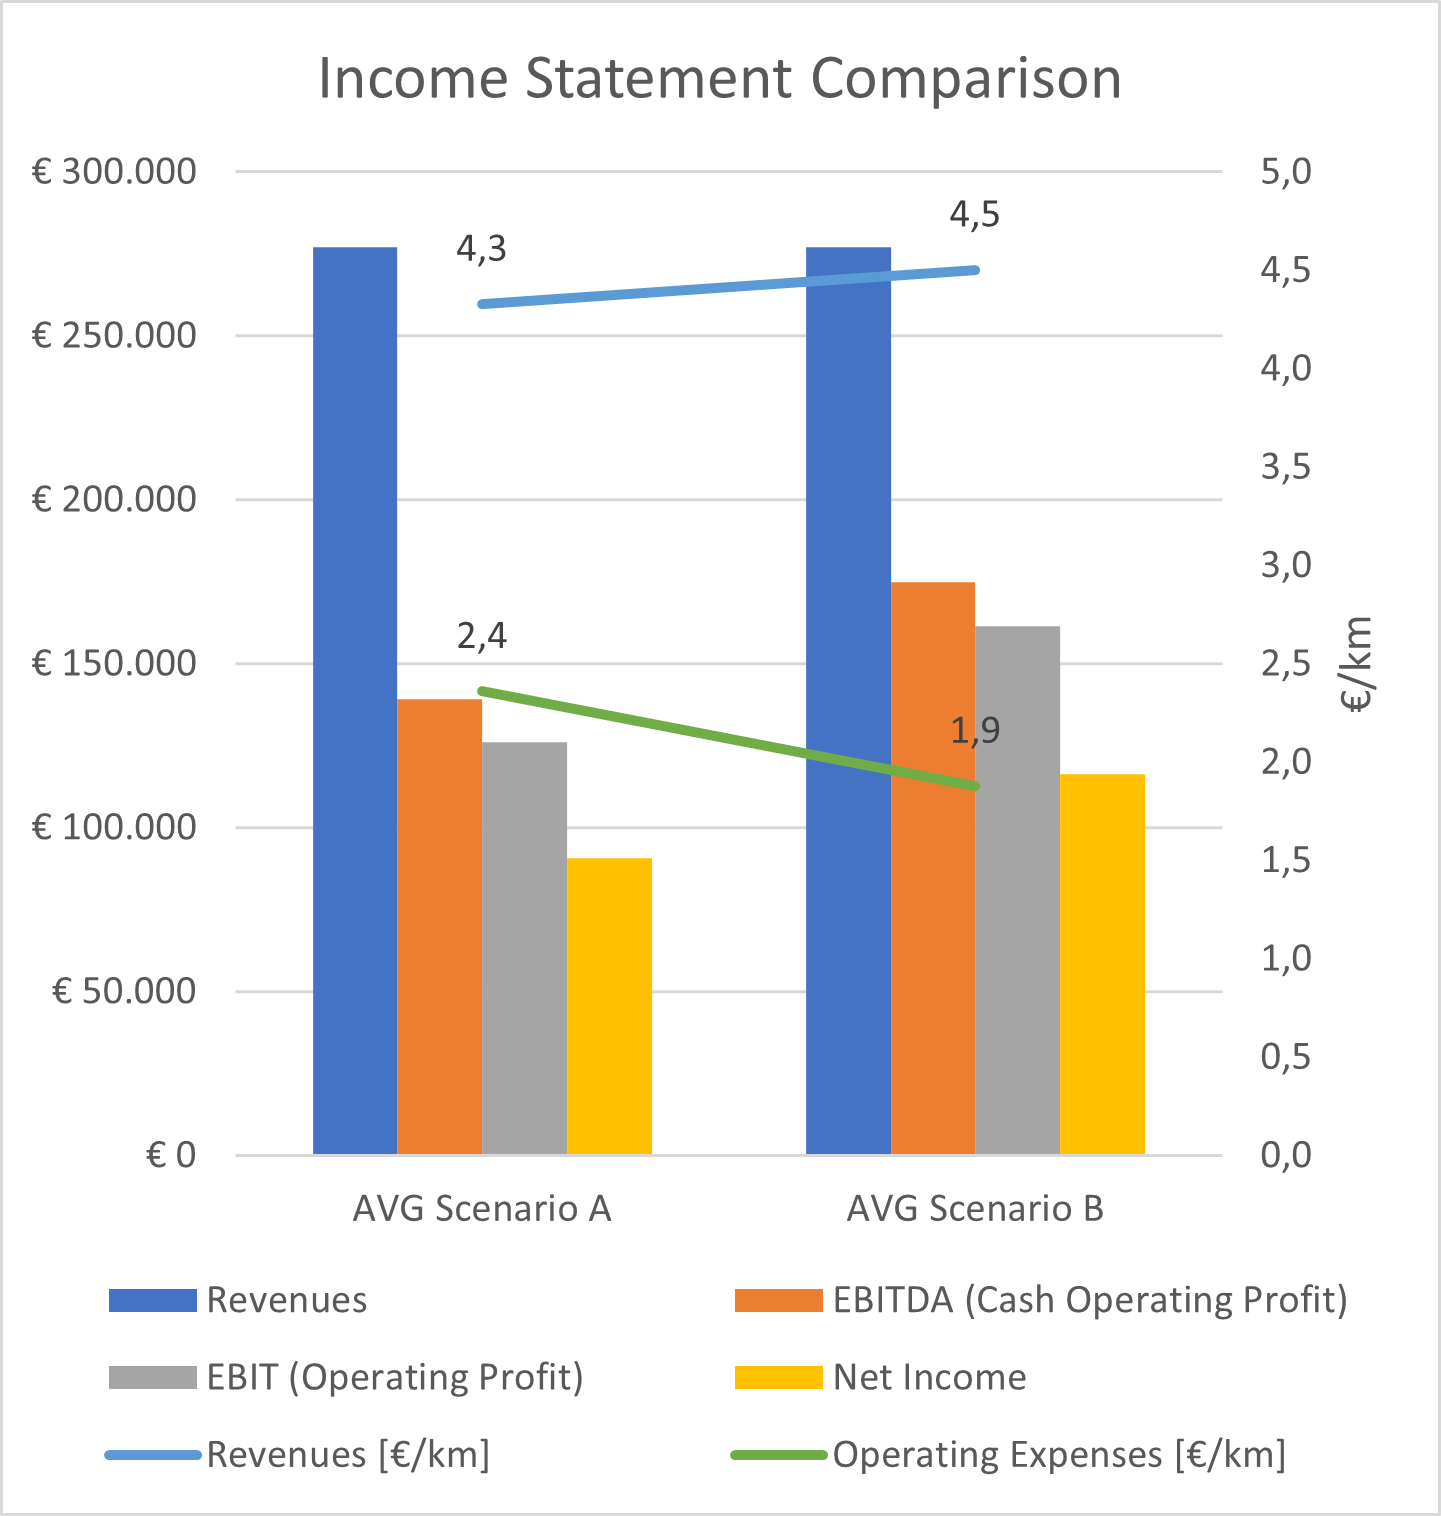
\includegraphics[width=0.7\textwidth]{Images/financial/Comparison.png}
    \caption{Income Statement Comparison}
    \label{fig:income_statement_comparison}
\end{figure}

\section{Sensitivity analysis}
This section will investigate the influence of some parameter’s variation, as “fuel cost” and the “passenger load”, over the economic performance. A cross analysis is performed to understand the combined power effect of the two above mentioned parameters, as a tool to understand the resilience of our business model to the last time world event (the higher passenger variability during the covid and after-covid period, combined with the energetic crisis due to the Ukraine war).

Because we select the hypothetical implementation of the scenario B, this analysis with be focused only on it.

The variability range used for the variables are:
\begin{itemize}
    \item +10\%, 0\%, - 10\% of the fuel cost
    \item +22\%, 0\%, -22\% of the mean passenger onboard (which means 34, 28, 22 travelling people)
\end{itemize}

On the offer side, the economic impact of the fuel cost variation described by the “Operating Cost”, is showed in the figure \ref{fig:opercost}.

\begin{figure}[h]
    \centering
    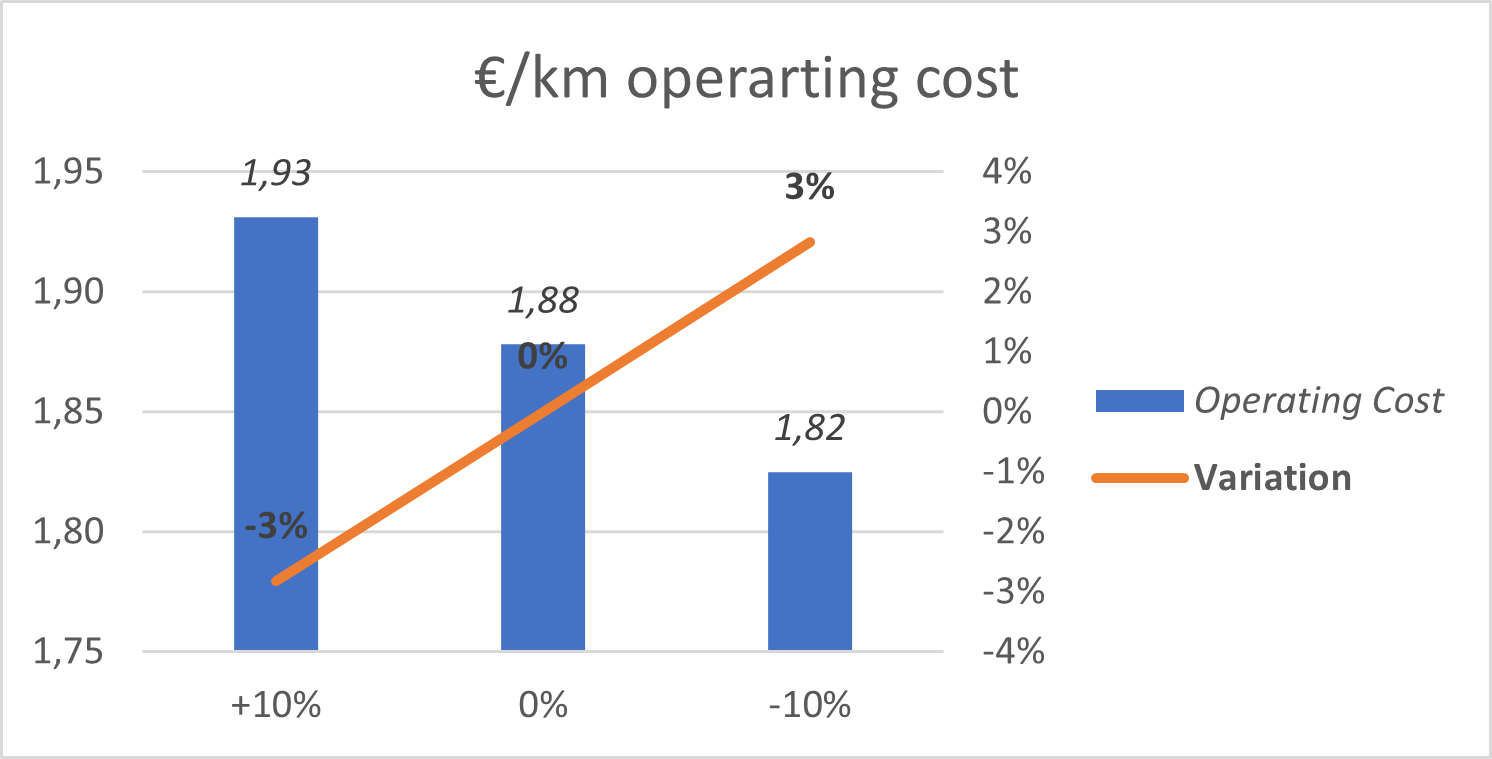
\includegraphics[width=0.7\textwidth]{Images/financial/operating_cost.png}
    \caption{Operating Cost}
    \label{fig:opercost}
\end{figure}

The consequent economic variation, in terms of “Delta EBIT” on percentage and distance metrics, is shown in figure \ref{fig:ebit},\ref{fig:ebitkm}.

\begin{figure}[h]
    \centering
    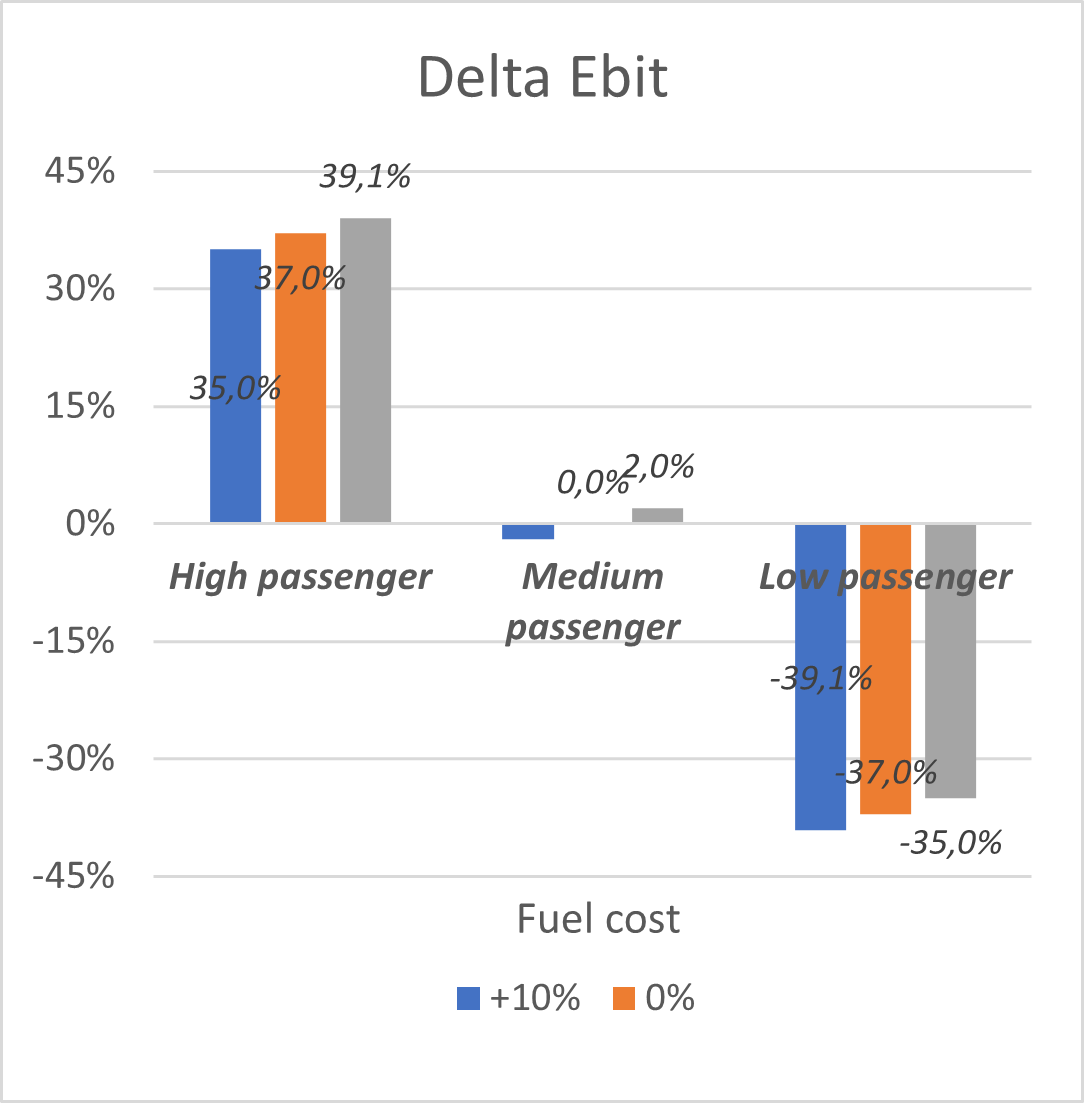
\includegraphics[width=0.7\textwidth]{Images/financial/ebitt.png}
    \caption{Delta EBIT}
    \label{fig:ebit}
\end{figure}

\begin{figure}[h]
    \centering
    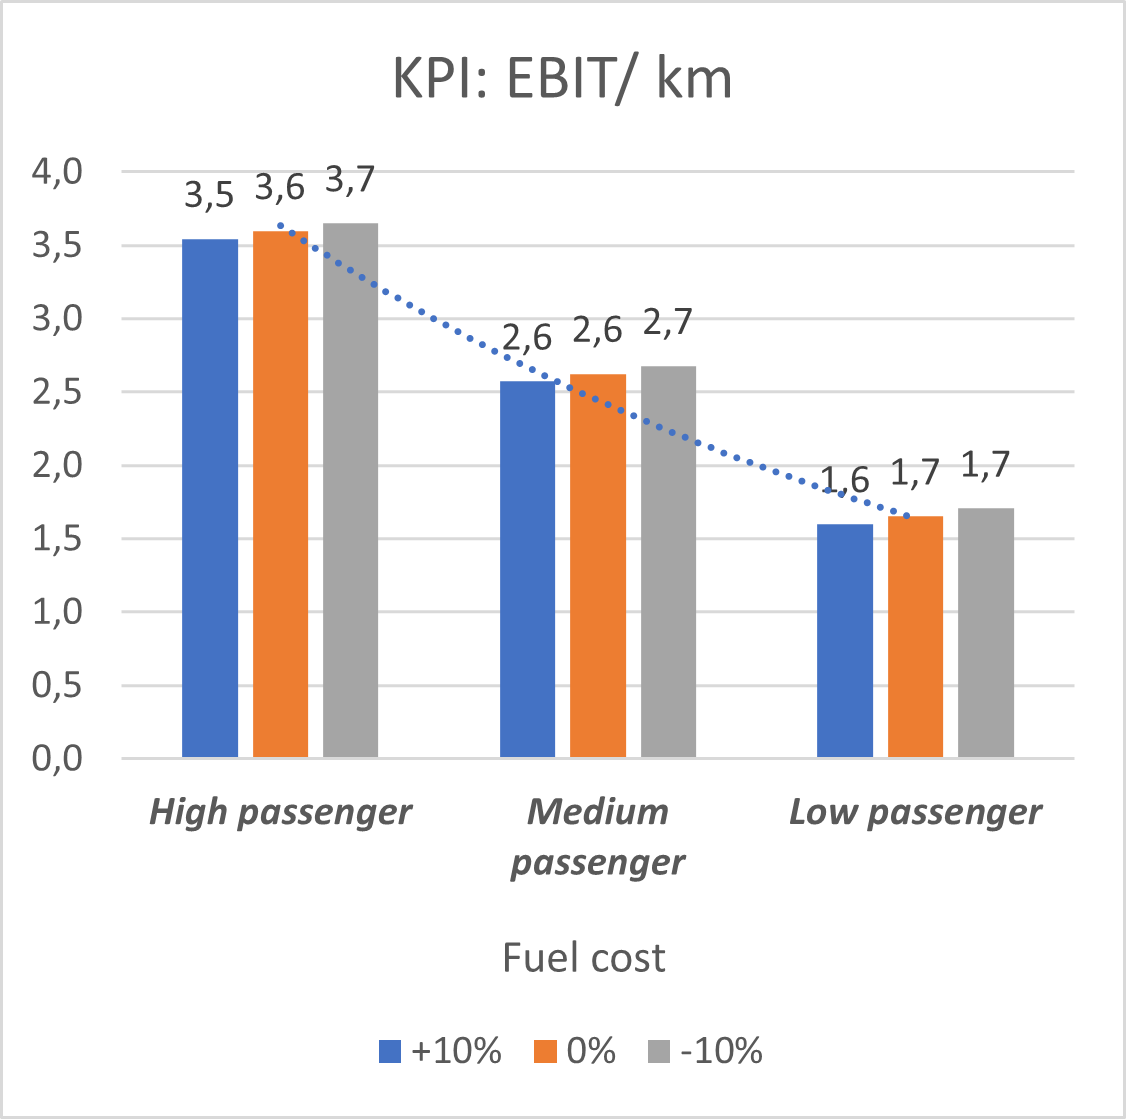
\includegraphics[width=0.7\textwidth]{Images/financial/ebitkm.png}
    \caption{EBIT/km}
    \label{fig:ebitkm}
\end{figure}

As is showed in these graphs, even in the “black-swan” scenario – increased fuel cost and the reduced number of passenger- our studied service is still able to generate cash from its operation, even if by 35\% less.

Lastly, give an average customer trip length of 33.2 km, even in the unrealistic case where all the on board passenger would be subscripted to seasonal ticket, the service would be still profitable, as represented in the table below.


\chapter{Marketing}

\epigraph{Dalla mattina alla sera,\\ da Stradella a Voghera.}{Slogan}
\section{An introduction to marketing strategies}
Setting up an effective marketing campaign is of paramount importance for a Company operating in any sector to launch a new product or service. The mobility sector is not an exception, a new transport service, even if properly scheduled, efficient under the O\&M point-of-view, and profitable on paper, remains under-utilized if potential customers don’t know about its existence.

The available budget for this kind of activities is often quite modest; therefore, the risk is to spend the resources in not an effective way, targeting the wrong customers or the wrong area.

The goal of this section is to present how the Team has decided to spend the $10000$ € budget made available by the company, explaining in detail the choices that guided the decisions, the selected marketing tools to make the people informed about the new service and finally what are the main KPI’s and how the Company could monitor the status of the campaign.

\paragraph{Target and area of interest}
Before starting with the actual marketing strategy, it is worth to carefully identify the border of the area that will be touched, along with the targets of the campaign.

The almost totality of the budget will be dedicated to the area of Pavia Province, mainly to the municipality of Voghera and to the Business Park area, where the launch event of the new service will take place (see next chapter).

Regarding the target, the strategy has as a goal to inform ideally each of the current employees and workers of the Park about the introduction of the new transport service. Being a service essentially dedicated to them, it has been considered convenient to reserve the largest part of the resources to the people that are spending their time inside the Business Park.

Therefore, a successful marketing campaign will be the one that persuades the largest number of employees to abandon their current mean of transport, to reach their workplace with the service offered by Autoguidovie. 

\paragraph{Market Strategy}
The selected strategy is a mix of “online” and “offline” tools revolving around a core event that will provide the participants the chance to touch with their hands the operability of the new service. The following scheme presents the structure of the entire strategy adopted.

\begin{figure}[h]
    \centering
    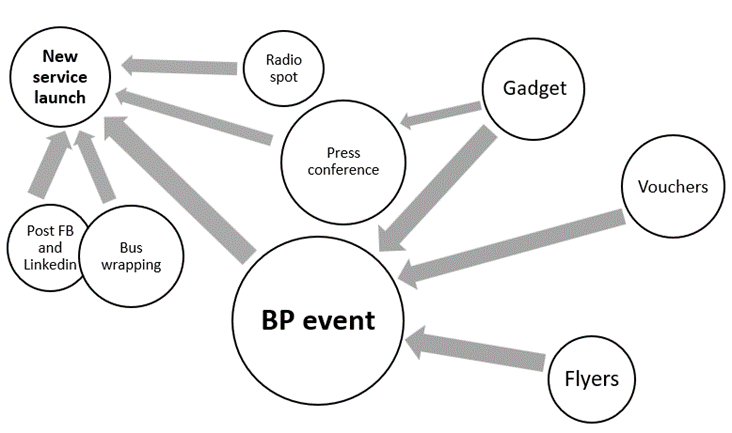
\includegraphics[width=0.7\textwidth]{Images/merketing/Strategy.png}
    \caption{Marketing Strategy}
    \label{fig:strategy}
\end{figure}

Each of the mentioned strategy, will be carefully described in a subsequent paragraph.

\section{KPI's and Costs of the strategies}
The initiatives abovementioned have obviously a cost for the Company, both in terms of financial resources and time to organize them. For this reason, it is fundamental to be able to monitor the effectiveness of these strategies through a proper set of KPI’s, to eventually adjust any decision that has previously been taken, and also to generate a record which could be useful for future marketing campaigns.

In the Table \ref{tab:marketing_strategy}, the reader can take a global look at the strategies, along with the KPI’s that have been selected for each of them and their budget.

\newpage
\thispagestyle{empty}
\begin{landscape}
\begin{table}[h]
\centering
\begin{tabular}{|l|l|l|l|l|}
\hline
\rowcolor{bluepoli!40}
\multicolumn{1}{|c|}{\textbf{Strategy}} & \multicolumn{1}{c|}{\textbf{Mode}} & \multicolumn{1}{c|}{\textbf{Cost}} & \multicolumn{1}{c|}{\textbf{Cost Composition}} & \multicolumn{1}{c|}{\textbf{KPI}} \\ \hline
Live BP Event                           & Offline                            & 5.000 \texteuro                             & -                                              & Used / Emitted   Voucher ratio    \\ \hline
CEO Press   Conference                  & Offline \&   Online                & 500 \texteuro                           & -                                              & Articles on local   news          \\ \hline
Bus Wrapping                            & Offline                            & 1.400  \texteuro                            & 70  \texteuro/bus $\cdot 20 bus$                        & -                                 \\ \hline
Local Radio Spots                       & Online                             & 294  \texteuro                              & 7  \texteuro/spot $\cdot 3   spot/day \cdot 14 day$     & Share                             \\ \hline
Social Media Posts                      & Online                             & 100  \texteuro                              & -                                              & N° of reactions                   \\ \hline
Flyers/Leaflets                         & Offline                            & 75  \texteuro                               & $0,75$  \texteuro/flyer $\cdot 100 flyer$                 & N° of participants at the event   \\ \hline
Vouchers                                & Online                             & 2105.4  \texteuro                          & 30\% expected revenues from monthly ticket     & Used / Emitted   Voucher ratio    \\ \hline
Gadget                                  & Offline                            & 450  \texteuro                             & $1.5 $ \texteuro/gadget $\cdot 300 gadget $               & -                                 \\ \hline
Survey                                  & Online                             & -                                  & -                                              & -                                 \\ \hline
\end{tabular}
\caption{Marketing Strategies description}
\label{tab:marketing_strategy}
\end{table}
\end{landscape}
\newpage

Each of the previous tools has a different timing for its implementation and for the monitoring of its KPI’s. This topic is addressed in a dedicated paragraph.
\section{A deep dive into the marketing strategy}
The main plan for our marketing strategy is an event at the Business Park where the potential customers can clearly understand in what our idea consists of and why they should consider it for their life as commuters. The live event consists in a catering at our cost that has the role of attractor for the event, followed by a brief presentation of the changes that the line from Voghera will have, with a particular focus on the extra rides added early in the morning and at 10 pm tailored for business park workers. The workers’ children could spend their time with an entertainer. The event ends with the delivery of a voucher for each participant which gives the right to a discount of 30\% for the first monthly subscription.

Moreover, the new bus, that the company must buy to ensure the service, can be exposed at the main entrance of the business park and it could offer a service on call for the ones that want to participate at the event. The event should take place on 8th October, which is the Saturday before the beginning of the service. The preparation to the event will begin at the beginning of September. This event should have a lump sum cost of around 5,000€, that is half of our marketing budget; this includes the catering, the rent for the location, family entertainment and the bus show and service.

The choice of investing a huge amount of money on this night is because we believe that this will be the most effective proposal among the possible ones. In fact, the reached target is really specific and the effort made for this event should convince great part of the workers. In addition to the budget for the event per se, the voucher discount will be covered by 2,105€ from the marketing budget. A "una tantum" cost of 800€ is included to take into account the administrative costs to put in service the voucher discount system. To evaluate the success of this proposal, the KPI selected is the ratio between the voucher activated and the participant to the event and, in a second moment, the subscriptions renewed by people that used the voucher. 

To advertise the event, the most effective way is through flyers that will be hanged up on message boards in the business park at the cost of 75€. Their success will be monitored by the presence at the event. 

A second way for communicating this new plan is to have a press conference the week before the start of the service in a rent room that will cost 500€. Journalist from local channels or newspapers such as ‘La Provincia Pavese’, ‘Il Punto’, ‘il Giorno’, ‘Voghera News’, ‘Milano Pavia TV’, ‘Telelombardia’, ‘TGR – Lombardia’ could be invited. The number of articles made about this conference could be useful to understand the spreading of this innovation. Both during the press conference and the catering, gadgets could be gifted such as pens or keychains. The production of these gadgets costs around 450€.

Finally, the last two ideas for spreading the news of this service in the province during the weeks before starting the service are: a radiophonic spot on Radio Voghera, which will cost around 300€ and the installation of bus wrapping on the side of the buses that should travel on the Voghera-Stradella line at the cost of 1,400€.


\section{Timings and KPIs Monitoring}

The launch of the new service is scheduled on the 10th of October, as previously mentioned. The marketing campaign starts six weeks before the launch of the service. The first two initiatives to be implemented are the publication of posts on social media, like Facebook and LinkedIn, and the wrapping on buses serving the line from Voghera to Stradella, line that will be modified for the Business Park service. The former is intended to reach the so called “white collars” of the Business Park, while the latter is targeting the pedestrians and drivers in the towns near the Business Park, that may come into contact with the wrapped buses. Both strategies start at the beginning of September to enhance the level of exposition and reach the highest number of potential customers. The wrapping process for 20 buses requires a week, thus the buses will be ready on 09/09. The posts on social media will be weekly monitored till the end of the marketing campaign, collecting the number of reactions and likes to measure the impact of the action.

The most institutional marketing measure for our stakeholders consists in a press conference on the 3/10; its preparation is estimated lasting 14 days, to find a location, invite journalists and set up the speech. During the press conference, gadgets will be distributed. They are made since the 11th September, to have 21 days of preparation and have them ready for the press event. The efficacy of the press will be monitored with the number of articles on the newspaper, weighted by the average number of copies sold.

The Business Park Live Event is organized two days before the New Service Launch, on a Saturday evening, to guarantee the highest participation of employees and workers. The estimated duration of its preparation is 35 days starting from the 03/09/22, to obtain the permission, find the catering and organize family entertainment during the evening. The effectiveness of this event is measured with two metrics: for the month of October with the ratio of used over emitted voucher, distributed during the event. For the month of November, on the other hand, the suggested KPI is the renovated monthly ticket over the original emitted voucher to get an indication of the initial customer loyalty for the new service.

Since the vouchers are distributed during the Live Event, and the expected duration for the administrative works is 21 days, their preparation starts on the 17/09/22.

Another item connected to the Live Event is the flyers. These will be hanged on boards inside the companies in the Business Park one week before the Live Event, and they require a week for their preparation.

The spots on Radio Voghera are scheduled for the last two weeks before the start of the new service in order to try to engage those who “were left behind” with the previous measures. Moreover, radiophonic spots can be effective to target a particular market segment: car users. 

Three spots per day are planned. The effectiveness of this action is measured by the average share of audience for each day on Radio Voghera during the spots airing.

For all the measures for which is difficult to find a synthetic KPI, like gadget and bus wrapping, surveys and interviews are suggested at the end of the Live Event and for the first weeks of the new bus service. These polls should enable the company to understand how customers got to know the new service and understand which measures were the most appreciated and effective ones, both from an advertising and economic perspective.


\begin{figure}[h]
    \centering
    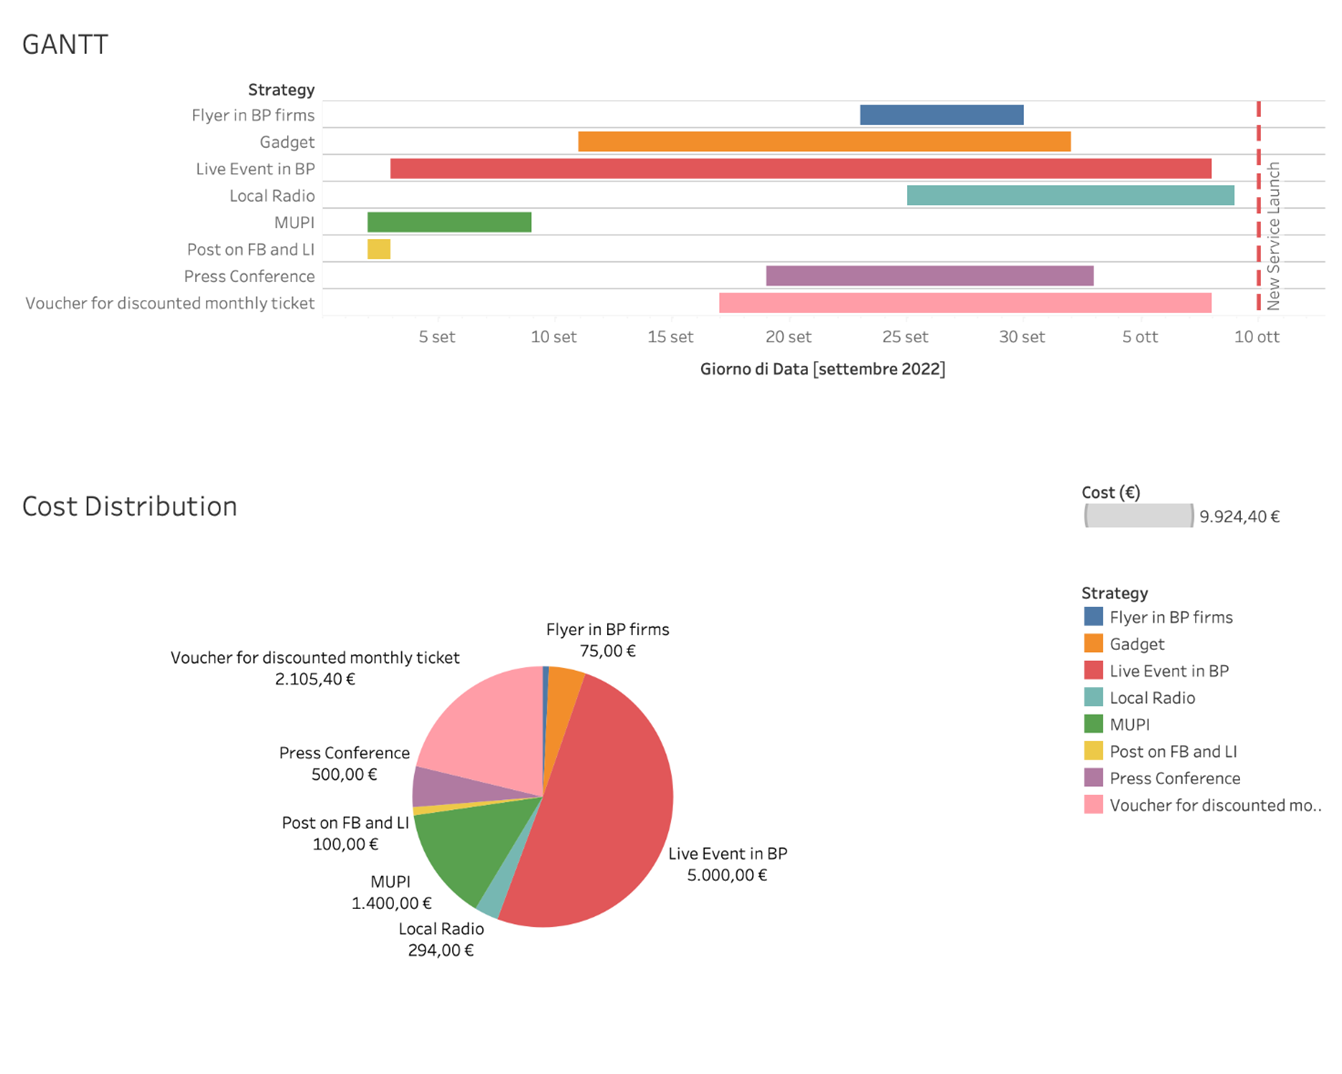
\includegraphics[width=0.7\textwidth]{Images/merketing/graph_marketing.png}
    \caption{GANTT Chart and Costs Distribution}
    \label{fig:gantt}
\end{figure}

%-------------------------------------------------------------------------
%	BIBLIOGRAPHY
%-------------------------------------------------------------------------

\addtocontents{toc}{\vspace{2em}} % Add a gap in the Contents, for aesthetics
\bibliography{references} % The references information are stored in the file named "Thesis_bibliography.bib"

%-------------------------------------------------------------------------
%	APPENDICES
%-------------------------------------------------------------------------

\cleardoublepage
\addtocontents{toc}{\vspace{2em}} % Add a gap in the Contents, for aesthetics
\chapter*{Appendix A}
\begin{algorithm}[H]
    \label{alg:Script}
    \caption{Algorithm made for the count of number of departure}
    \label{alg:var}
    \label{protocol1}
    \begin{algorithmic}[1]
    \STATE{Import in case of Python pandas, numpy, datetime, pathlib}
    \STATE{Import  the Rides$\_$list.xlsx file and clean columns and data hour format}
    \STATE{Build the output dataframe with the first column the route code}
    \FOR{$each\, timeslot$}
    \STATE{add a column in the output dataset}
    \STATE{Count the occurencies of the values and update the dataset}
    \ENDFOR
    \STATE Export the dataset
    \end{algorithmic}
\end{algorithm} 



% LIST OF FIGURES
\listoffigures

% LIST OF TABLES
\listoftables
\end{document}
